%==============================================================================
%  DisloCluster User Manual
%
%  Standalone, single-file document. No external figures: all diagrams are TikZ.
%  Compiles with pdflatex; also fine on Overleaf.
%
%  Replaces the operating appendix of "Zr3d Code Architecture", which was
%  written for the earlier two-repository layout (Fluor_Zr + MoDELib).
%  This manual is written against the unified DisloCluster repository:
%      https://github.com/Ghoniem/DisloCluster
%==============================================================================
\documentclass[11pt]{article}

% Type1 outlines for the whole EC/TC family. Without these the document falls
% back to OT1 Computer Modern, and the first text-companion glyph asks MiKTeX
% to build a bitmap font with METAFONT -- which fails here with
% "This can't happen (copy)" on tctt0900 and takes the build down with it.
% solver_and_coupling_rearchitecture.tex has carried these three lines from the
% start, which is why it compiles cleanly and this document did not.
\usepackage[T1]{fontenc}
\usepackage[utf8]{inputenc}
\usepackage{lmodern}

\usepackage[margin=1in]{geometry}
\usepackage{amsmath,amssymb}
\usepackage{booktabs}
\usepackage{longtable}
\usepackage{array}
\usepackage{graphicx}
\usepackage{xcolor}
\usepackage{listings}
\usepackage{tikz}
\usepackage{hyperref}
\usetikzlibrary{arrows.meta,positioning,fit,backgrounds,calc,shapes.geometric}

\hypersetup{colorlinks=true,linkcolor=blue!50!black,urlcolor=blue!50!black,
            citecolor=blue!50!black}

\setcounter{secnumdepth}{4}
\setcounter{tocdepth}{2}
\emergencystretch=2.5em

% ---- shorthands -------------------------------------------------------------
\newcommand{\aloop}{\ensuremath{\langle a\rangle}}
\newcommand{\cloop}{\ensuremath{\langle c\rangle}}
\newcommand{\ZrM}{\textsf{ZrMicro}}
\newcommand{\MoD}{\textsf{MoDELib3}}
\newcommand{\DC}{\textsf{DisloCluster}}
\newcommand{\code}[1]{\texttt{\small #1}}
\newcommand{\file}[1]{\texttt{\footnotesize #1}}

% ---- code listing styles ----------------------------------------------------
\lstset{basicstyle=\ttfamily\footnotesize,
        breaklines=true,
        columns=fullflexible,
        frame=single,
        framesep=4pt,
        rulecolor=\color{black!30},
        backgroundcolor=\color{black!3},
        showstringspaces=false,
        keepspaces=true}

% PowerShell (Windows) listings: light blue frame
\lstdefinestyle{ps}{rulecolor=\color{blue!35},backgroundcolor=\color{blue!3}}
% WSL / bash listings: light green frame
\lstdefinestyle{wsl}{rulecolor=\color{green!45!black!40},backgroundcolor=\color{green!5}}
% Python listings
\lstdefinestyle{py}{language=Python,rulecolor=\color{black!30},backgroundcolor=\color{black!3}}

% ---- callout boxes ----------------------------------------------------------
\newenvironment{warnbox}
  {\par\medskip\noindent
   \begin{minipage}{\textwidth}
   {\color{red!60!black}\rule{\textwidth}{0.8pt}}\par\smallskip
   \small\noindent{\color{red!60!black}\textbf{Warning.}}\space}
  {\par\smallskip\noindent{\color{red!60!black}\rule{\textwidth}{0.8pt}}
   \end{minipage}\par\medskip}

\newenvironment{notebox}
  {\par\medskip\noindent
   \begin{minipage}{\textwidth}
   {\color{blue!50!black}\rule{\textwidth}{0.8pt}}\par\smallskip
   \small\noindent{\color{blue!50!black}\textbf{Note.}}\space}
  {\par\smallskip\noindent{\color{blue!50!black}\rule{\textwidth}{0.8pt}}
   \end{minipage}\par\medskip}

% ---- flowchart palette ------------------------------------------------------
\definecolor{cNotebook}{RGB}{ 33, 87,150}   % orchestration
\definecolor{cPy}      {RGB}{ 45,125, 90}   % ZrMicro python
\definecolor{cCpp}     {RGB}{155, 60, 30}   % ZrMicro C++
\definecolor{cMod}     {RGB}{110, 55,140}   % MoDELib C++
\definecolor{cData}    {RGB}{140,110, 20}   % files on disk
\definecolor{cOut}     {RGB}{ 70, 70, 70}   % products

\title{\textbf{DisloCluster User Manual}\\[6pt]
\large Installation, Build, and Simulation Guide\\
\large Coupled Cluster Dynamics -- Dislocation Dynamics of Irradiated Zirconium}
\author{Nasr M.\ Ghoniem}
\date{\today\\[4pt]\normalsize Repository: \url{https://github.com/Ghoniem/DisloCluster}}

\begin{document}
\maketitle

\begin{abstract}
\noindent
\DC{} simulates radiation effects in zirconium by coupling a zero-dimensional
(0-D) reduced cluster-dynamics model of point-defect and dislocation-loop
evolution (\ZrM{}) to a three-dimensional, spatially resolved
cluster-dynamics / dislocation-dynamics code (\MoD{}, a fork of
MoDELib-fullCD). This manual takes a user from a fresh clone of the repository
on a new Windows machine to a completed simulation: installing the
prerequisites (Section~\ref{sec:install}), creating the Python virtual
environment (Section~\ref{sec:venv}), compiling the two C++ codes
(Section~\ref{sec:build}), and running the three kinds of simulation the
repository supports --- the standalone 3-D single-crystal test
(Section~\ref{sec:first}), the 0-D \ZrM{} model (Section~\ref{sec:zeroD}),
and the coupled 0-D$\,\leftrightarrow\,$3-D dose march
(Section~\ref{sec:coupled}). Section~\ref{sec:changing} explains where to
change physical and numerical parameters, Section~\ref{sec:trouble} collects
the known failure modes and their fixes, and Section~\ref{sec:repro}
describes the provenance system that makes every run reproducible.
Appendix~\ref{app:arch} is a condensed architecture reference,
Appendix~\ref{app:changes} summarizes the physics added relative to the
upstream MoDELib-fullCD code, and Appendix~\ref{app:quickref} is a one-page
command summary.
\end{abstract}

\tableofcontents
\clearpage

%==============================================================================
\section{Introduction}
\label{sec:intro}

\subsection{What \DC{} does}

Irradiated zirconium develops a microstructure of prismatic \aloop{}
interstitial loops and basal \cloop{} vacancy loops, fed by the point defects
(vacancies, single interstitials, di- and tri-interstitials) that displacement
cascades produce. The physics splits into two widely separated time scales:
the \emph{mobile} point-defect species relax to their local sink environment
in milliseconds, while the \emph{immobile} loop populations evolve over dose
steps of order $10^{7}$~s. \DC{} exploits that split with an operator-split
quasi-steady-state (QSSA) scheme: within each dose step the fast mobile
species are solved as a steady reaction--diffusion field, and the slow loop
populations are then marched in dose against the frozen mobile field.

The repository contains two codes that realize this physics at different
levels of spatial resolution, plus the coupling layer between them:

\begin{itemize}
\item \textbf{\ZrM{}} (\file{ZrMicro/}) --- the 0-D reduced
model: 19 coupled ODEs (12 physical species, 6 conservation accumulators, and
the evolving network dislocation density $\rho_N$), integrated with SUNDIALS
CVODE through a compiled C++ solver, orchestrated and post-processed in
Python.
\item \textbf{\MoD{}} (\file{MoDELib3/}) --- the 3-D spatially resolved
cluster-dynamics / dislocation-dynamics code: a finite-element solver for the
steady mobile boundary-value problem and a pointwise dose march for the four
loop families, run by the \code{DDomp} executable.
\item \textbf{The coupling layer} (\file{dislocluster\_code/coupling/} and
the notebook \file{Simulations/run\_simulation.ipynb}) --- exchanges the
per-node immobile field and the steady mobile field between the two codes
over a shared dose schedule.
\end{itemize}

\subsection{The three ways to run it}
\label{sec:threeways}

Everything in this manual funnels into one of three simulation types, and it
is worth fixing them in mind now:

\begin{enumerate}
\item \textbf{The 3-D single-crystal run} (Section~\ref{sec:first}) --- a
standalone \MoD{} simulation of a 1~$\mu$m cubic grain under irradiation,
driven by a shell script. No Python is involved in the solve. This is the
recommended first test on a new machine, because the repository ships with
the results of a completed solve (\file{evl/}), so the post-processing can be
exercised in minutes, before the hours-long solve is attempted.
\item \textbf{The 0-D \ZrM{} run} (Section~\ref{sec:zeroD}) --- the reduced
model alone, driven by the notebook \file{ZrMicro.ipynb}. Fast (minutes), and
the source of the fitted parameter set.
\item \textbf{The coupled 0-D$\,\leftrightarrow\,$3-D march}
(Section~\ref{sec:coupled}) --- the operator-split coupling, driven by the
notebook \file{Simulations/run\_simulation.ipynb}. Python owns the dose loop,
\MoD{} solves the fast mobile field, and the \ZrM{} C++ integrator marches
the immobile state at every quadrature point. This is the normal entry point
for new work; the older \file{coupled\_0d\_3d\_ZrMicro.ipynb} carries its own
inline copy of the march and is kept only for reference.
\end{enumerate}

\begin{notebox}
\textbf{Updated (14 August 2026).} The Python was gathered into one installed
package, \file{dislocluster\_code/}, and simulations moved to
\file{Simulations/}, which now holds \file{input/} and \file{output/} beside
the notebooks the way \file{ZrMicro/} used to. \file{ZrMicro/py\_utils/}
survives as a shim: every former module is an alias for its new home, so
\code{from py\_utils import paths} and \code{python -m py\_utils.X} still
work. Runs made before the move stay under \file{ZrMicro/output/} and are
still found, because \code{paths.find\_runs()} searches every output root.
\end{notebox}

\subsection{Repository layout}
\label{sec:layout}

The repository is self-contained: nothing outside the repository root is
required except the Python interpreter, SUNDIALS, and (on Windows) WSL. The
layout is:

\begin{lstlisting}
DisloCluster/                    <- repository root (.dislocluster_root marker)
|- .DisloClusterVenv/            Python 3.14 environment (you create this)
|- Libraries/                    SUNDIALS install location (you create this)
|  \- sundials-7.1.1/
|- requirements.txt              pinned environment lock
|- pyproject.toml                the package (pip install -e .)
|- dislocluster_code/            ALL Python lives here
|  |- paths.py                   single source of truth for every location
|  |- config.py                  SimulationConfig: the notebook's six dicts
|  |- driver.py                  prepare / march / report
|  |- build.py                   ensure_zrmicro_solver, ensure_modelib
|  |- zerod/                     the 0-D model chain
|  |- staging/                   mesh, input files, seed, bootstrap
|  |- coupling/                  the operator split, checkpoint, progress
|  |- post/                      figures, movies, discrete loops, reports
|  \- studies/ fitting/ legacy/  comparison drivers, fits, superseded code
|- Simulations/                  WHERE SIMULATIONS ARE RUN
|  |- run_simulation.ipynb       <- the normal entry point
|  |- postprocess.ipynb          re-render an existing run
|  |- input/                     the Excel parameter workbooks
|  \- output/                    timestamped run directories
|- Gmsh/                         generate_mesh.py + meshes/ cache
|- Docs/
|  |- DisloCluster Manual/       this manual
|  \- Formulation/               formulation documents + build_modelib.sh
|- ZrMicro/                      0-D side, C++ only now
|  |- code/                      solver.cpp + the older notebooks
|  |  |- ZrMicro.ipynb           0-D run + parameter identification
|  |  \- coupled_0d_3d_ZrMicro.ipynb   superseded by Simulations/
|  |- cpp_utils/                 C++ RHS + CMake build (SUNDIALS CVODE)
|  |- py_utils/                  compatibility shim -> dislocluster_code
|  |- input/                     older workbook copies (not read)
|  |- build/                     compiled solver.exe (created by the build)
|  \- output/                    runs made before Simulations/output/ existed
\- MoDELib3/                     3-D side (fork of MoDELib-fullCD)
   |- Library/Materials/         Zr3d_ghoniem.txt is the coupled material
   |- tutorials/                 staged simulation cases + the reference case
   \- build/                     DDomp + pyMoDELib (built inside WSL)
\end{lstlisting}

Nothing in the repository hard-codes an absolute path. The single source of
truth for every location is the module
\begin{center}
\file{dislocluster\_code/paths.py}
\end{center}
which finds the repository root by walking up to the
\file{.dislocluster\_root} marker, so the repository can be cloned or moved
anywhere. Three optional environment variables override the defaults:
\code{DISLOCLUSTER\_ROOT} (repository root), \code{MODELIB\_ROOT} (a \MoD{}
checkout outside the tree), and \code{MODELIB\_BUILD} (its build directory).

\begin{notebox}
\textbf{Resolved (8 August 2026).} \file{README.md}, the \file{CLAUDE.md}
files and \file{paths.py} used to refer to the formulation documents and the
WSL build script as living under \file{Docs/}. No such
folder exists --- all documents are under \file{Docs/} at the
\emph{repository root} --- and the stale references had produced two live
faults, both now fixed:
\begin{itemize}
  \item \file{paths.py} defined \code{DOCS\_DIR} as
        \file{Docs/Formulation}, so
        \code{MODELIB\_BUILD\_SCRIPT} pointed at a non-existent file and the
        coupling notebook's automatic \MoD{} build silently declined to run
        (it tests \code{is\_file()} and returns without comment).
        \code{DOCS\_DIR} is now the root \file{Docs/}, with
        \code{DOCS\_FORMULATION} and \code{DOCS\_MANUAL} beside it.
  \item \file{build\_modelib\_wsl.sh} (now \file{build\_modelib.sh}) derived the repository root by walking
        up three directories, correct only from the old location
        (Section~\ref{sec:buildmod}).
\end{itemize}
\end{notebox}

\subsection{Conventions used in this manual}

The primary platform is Windows~11 with WSL\,2 (Ubuntu): \ZrM{} builds and
runs natively on Windows, while \MoD{} is built and executed inside WSL,
because it needs a GNU toolchain, Eigen, FFTW and SuiteSparse. Command blocks
are colour-coded:

\begin{lstlisting}[style=ps]
PS>  a Windows PowerShell command, run from the repository root
\end{lstlisting}

\begin{lstlisting}[style=wsl]
$    a bash command inside WSL (or any Linux shell)
\end{lstlisting}

On a native Linux or macOS machine the same steps apply with the obvious
simplifications: there is no WSL boundary, both codes build in the same
shell, the venv lives at \file{.DisloClusterVenv/bin/}, and
\file{paths.py} automatically selects the native binaries.

%==============================================================================
\section{Installation}
\label{sec:install}

\subsection{Prerequisites}

Table~\ref{tab:prereq} lists everything the repository needs. The rest of
this section walks through installing each item in order.

\begin{table}[htbp]
\centering
\caption{Prerequisites. Windows-side tools build and run \ZrM{}; WSL-side
tools build and run \MoD{}.}
\label{tab:prereq}
\small
\begin{tabular}{@{}p{0.28\textwidth}lll@{}}
\toprule
component & version & side & purpose \\
\midrule
Git & any recent & Windows & clone the repository \\
Python & 3.14 (python.org) & Windows & venv, notebooks, orchestration \\
VS Build Tools & 2022 (C++ workload) & Windows & compile \ZrM{} \\
CMake & $\ge 3.16$ & Windows & configure \ZrM{} and SUNDIALS \\
SUNDIALS & 7.1.1 & Windows & CVODE/ARKODE for \ZrM{} \\
WSL\,2 + Ubuntu & 22.04 or 24.04 & WSL & build and run \MoD{} \\
apt packages & Sec.~\ref{sec:buildmod} & WSL & installed by the build script \\
\bottomrule
\end{tabular}
\end{table}

\begin{warnbox}
\textbf{Do not use Anaconda Python} for this project. Its NumPy~1.x/2.x mix
conflicts with the SciPy pinned in \file{requirements.txt}. Install CPython
3.14 from \url{https://www.python.org} and build the venv from that
interpreter.
\end{warnbox}

\subsection{Step 1: Windows tools}

\begin{enumerate}
\item \textbf{Git for Windows} --- \url{https://git-scm.com}. Default options
are fine.
\item \textbf{Python 3.14} --- \url{https://www.python.org/downloads/}.
Install for all users (the manual assumes \file{C:\textbackslash
Python314\textbackslash python.exe}; adjust paths if you install elsewhere).
It is not necessary to add it to \code{PATH} --- every command in this manual
calls an interpreter by explicit path.
\item \textbf{Visual Studio 2022 Build Tools} ---
\url{https://visualstudio.microsoft.com/downloads/}, workload
``Desktop development with C++''. This provides the MSVC compiler and the
OpenMP runtime that \ZrM{}'s parallel batch mode uses.
\item \textbf{CMake} --- \url{https://cmake.org/download/}, and let the
installer add it to \code{PATH}. Any CMake $\ge 3.16$ works for the
Windows-side builds.
\end{enumerate}

\subsection{Step 2: clone the repository}

From the directory that should contain the repository (any location works;
no path is hard-coded):

\begin{lstlisting}[style=ps]
PS> git clone https://github.com/Ghoniem/DisloCluster.git
PS> cd DisloCluster
\end{lstlisting}

The repository is private, so the clone authenticates with your GitHub
account (Git for Windows will pop up a browser-based credential prompt the
first time).

All subsequent commands in this manual are issued \emph{from the repository
root} unless stated otherwise.

\begin{notebox}
\DC{} was assembled from two previously separate repositories, which were
submodules until commit \code{859af47} converted them to plain directories.
It is now a single git checkout. The root marker file
\file{.dislocluster\_root} --- not any \file{.git} --- is what identifies the
repository root to \file{paths.py}, and \code{paths.git\_hash()} still falls
back through root $\rightarrow$ \file{ZrMicro} $\rightarrow$ \file{MoDELib3}
so that a split checkout would keep producing meaningful provenance tags.
\end{notebox}

\subsection{Step 3: WSL and Ubuntu}
\label{sec:wslinstall}

\MoD{} needs a Linux toolchain. On Windows this is provided by WSL\,2:

\begin{lstlisting}[style=ps]
PS> wsl --install
\end{lstlisting}

Reboot when prompted, then complete the Ubuntu first-run setup (create a
Linux username and password). Verify:

\begin{lstlisting}[style=ps]
PS> wsl -e bash -c "lsb_release -d && gcc --version | head -1"
\end{lstlisting}

The compilers and libraries \MoD{} needs inside WSL are installed
automatically by the build script in Section~\ref{sec:buildmod}; nothing
further is required here.

\subsection{Step 4: SUNDIALS 7.1.1}
\label{sec:sundials}

\ZrM{}'s C++ solver links against SUNDIALS 7.1.1 (modules \code{cvode},
\code{arkode}, \code{nvecserial}, \code{sunlinsolband},
\code{sunlinsolspgmr}). The \ZrM{} CMake build looks for it in two places, in
order: \file{$\langle$repo$\rangle$/Libraries/\allowbreak sundials-7.1.1/}
(preferred),
then the system-wide CMake package registry (e.g.\ an install under
\file{C:\textbackslash Program Files (x86)\textbackslash SUNDIALS}).

To build and install it into the repository tree (recommended --- it keeps
the whole project self-contained), run from a scratch directory:

\begin{lstlisting}[style=ps]
PS> curl.exe -LO https://github.com/LLNL/sundials/releases/download/v7.1.1/sundials-7.1.1.tar.gz
PS> tar -xzf sundials-7.1.1.tar.gz
PS> cmake -S sundials-7.1.1 -B sundials-build `
      -DCMAKE_INSTALL_PREFIX="<path-to>\DisloCluster\Libraries\sundials-7.1.1" `
      -DBUILD_SHARED_LIBS=OFF -DBUILD_STATIC_LIBS=ON `
      -DEXAMPLES_ENABLE_C=OFF -DEXAMPLES_INSTALL=OFF
PS> cmake --build sundials-build --config Release --target install
\end{lstlisting}

Replace \file{<path-to>} with the actual location of your clone. The install
step populates \file{Libraries/sundials-7.1.1/} with \file{include/},
\file{lib/} and the CMake package files that \code{find\_package(SUNDIALS)}
consumes.

%==============================================================================
\section{The Python virtual environment}
\label{sec:venv}

\subsection{Create the venv and install dependencies}

The whole repository shares one virtual environment,
\file{.DisloClusterVenv/}, at the repository root. From the repository root:

\begin{lstlisting}[style=ps]
PS> C:\Python314\python.exe -m venv .DisloClusterVenv
PS> .DisloClusterVenv\Scripts\python.exe -m pip install -r requirements.txt
\end{lstlisting}

\file{requirements.txt} pins the full stack --- NumPy~2.4, SciPy~1.17,
pandas, Matplotlib, openpyxl (the Excel workbook reader), the Gmsh SDK (mesh
generation for the Adaptive notebook), and the complete JupyterLab toolchain
--- so the install is reproducible on any machine.

\subsection{Register the Jupyter kernel}

The notebooks expect a kernel named \code{dislocluster}:

\begin{lstlisting}[style=ps]
PS> .DisloClusterVenv\Scripts\python.exe -m ipykernel install --user `
      --name dislocluster --display-name "Python 3.14 (DisloCluster)"
\end{lstlisting}

When a notebook is opened in JupyterLab or VS~Code, select the kernel
``Python 3.14 (DisloCluster)''.

\subsection{Verify path resolution}
\label{sec:pathsverify}

Before building anything, confirm that the path-resolution layer sees your
checkout correctly:

\begin{lstlisting}[style=ps]
PS> .DisloClusterVenv\Scripts\python.exe dislocluster_code\paths.py
\end{lstlisting}

This prints one \code{OK}/\code{MISS} line per resolved location (repository
root, venv, 0-D code, solver binary, \MoD{} root and build, material file,
coupled simulation case, \dots). At this stage \code{MISS} is expected for
the two solver binaries --- they have not been built yet --- and everything
else should read \code{OK}. Re-run this command whenever something cannot be
found; it is the fastest diagnostic in the repository.

%==============================================================================
\section{Building the two codes}
\label{sec:build}

\subsection{The 0-D \ZrM{} solver (Windows, native)}
\label{sec:buildzrm}

From the repository root:

\begin{lstlisting}[style=ps]
PS> cmake -S ZrMicro\cpp_utils -B ZrMicro\build `
      -DCMAKE_BUILD_TYPE=Release
PS> cmake --build ZrMicro\build --config Release
\end{lstlisting}

This produces \file{ZrMicro\textbackslash build\textbackslash
Release\textbackslash solver.exe}. Use \code{Release}:
the parameter-identification utilities call the solver thousands of times,
and the OpenMP batch mode --- which the Adaptive march relies on --- is only
worth having when optimized. OpenMP is detected automatically by CMake; the
solver still builds and runs serially without it, and the configure output
says which happened
(\code{OpenMP enabled for solver (parallel batch mode)} or
\code{OpenMP NOT found}).

If CMake cannot find SUNDIALS, check that the install prefix of
Section~\ref{sec:sundials} is exactly
\file{$\langle$repo$\rangle$/Libraries/sundials-7.1.1/}; that path is the
first entry on the build's \code{CMAKE\_PREFIX\_PATH}.

\subsection{The 3-D \MoD{} code}
\label{sec:buildmod}

\MoD{} is built by the script \file{Docs/Formulation/build\_modelib.sh},
which installs the dependencies its platform needs, discards any build cache
configured under a different absolute path (which is what happens when a
checkout is moved), and builds the headless targets. The same script serves
Linux, macOS and WSL; only the launcher differs. From the repository root:

\begin{lstlisting}[style=ps]
PS> wsl -u root -e bash Docs/Formulation/build_modelib.sh MoDELib3
\end{lstlisting}
\begin{lstlisting}[style=wsl]
$ bash Docs/Formulation/build_modelib.sh MoDELib3   # Linux, macOS, WSL shell
\end{lstlisting}

\begin{notebox}
\textbf{Fixed (8 August 2026).} The script's no-argument default used to walk
up \emph{three} directories from its own location, which was correct only
while it sat at \file{Docs/Formulation/}. From
\file{Docs/Formulation/} --- two levels below the root --- that resolved one
directory \emph{above} the checkout, and the script stopped with
``\code{CMakeLists.txt not found}''. Only the explicit-argument path, which
the coupling notebook uses, still worked. It now walks up two levels, so the
no-argument form works again:
\begin{lstlisting}[style=ps]
PS> wsl -u root -e bash Docs/Formulation/build_modelib.sh
\end{lstlisting}
Passing \file{MoDELib3} explicitly remains unambiguous from any location.
(Running as \code{-u root} avoids an interactive \code{sudo} password prompt
for the package installs.)
\end{notebox}

The script performs, in order:
\begin{enumerate}
\item Dependency installation through whichever package manager the platform
has --- \code{apt-get}, \code{dnf} or \code{pacman} on Linux, Homebrew on
macOS --- covering the toolchain, \code{cmake}, \code{ninja}, Eigen, OpenMP,
FFTW, SuiteSparse, Boost and pybind11. Set \code{SKIP\_DEPS=1} to skip this
step when the libraries are already in place. Only a C++20 compiler, CMake
$\ge 3.16$ and Eigen 3 are required; everything else is optional and its
absence is reported in the configuration summary rather than fatal.
\item Stale-cache detection: if \file{build/CMakeCache.txt} was configured
for a different source path (a moved or copied checkout), the build tree is
removed and reconfigured cleanly.
\item Configure and build: \code{Release}, Ninja when it is installed and the
default generator otherwise, with \code{-j} set from the core count
(\code{nproc} on Linux, \code{sysctl} on macOS).
\end{enumerate}

\begin{notebox}
\textbf{Changed.} The script was \file{build\_modelib\_wsl.sh} and, on every
run, \code{sed}-patched the inherited \file{CMakeLists.txt}: rewriting the
Eigen include path to Debian's \file{/usr/include/eigen3}, deleting the macOS
Qt and MacPorts RPATH lines, and commenting \code{add\_subdirectory(DDqt)} out
of \file{tools/CMakeLists.txt}. The source tree therefore carried whichever
platform's edits had been applied last, and the committed CMakeLists could
only build on Linux. The CMake files now make those decisions themselves ---
each dependency is searched for, each optimization flag is probed against the
compiler in hand, \code{DDqt} is built when Qt6 and VTK are found --- so one
script and one CMakeLists serve Linux, WSL and macOS alike. The
\code{-DCMAKE\_POLICY\_VERSION\_MINIMUM=3.5} workaround is gone with it:
\code{cmake\_minimum\_required} is now 3.16, which CMake~4 accepts directly.
\end{notebox}

The build takes 10--30 minutes from clean. Its artifacts are
\file{MoDELib3/build/tools/\allowbreak DDomp/DDomp} (a native executable ---
invoked directly on Linux and macOS, and from Windows through \code{wsl.exe},
which \code{paths.ddomp\_cmd()} decides per platform) and
\file{MoDELib3/build/tools/\allowbreak pyMoDELib/pyMoDELib*.so} (optional
Python bindings, built only when pybind11 is installed).

\subsection{Verify the builds}

Re-run the resolution report of Section~\ref{sec:pathsverify}:

\begin{lstlisting}[style=ps]
PS> .DisloClusterVenv\Scripts\python.exe dislocluster_code\paths.py
\end{lstlisting}

The rows \code{0-D solver} and \code{MoDELib DDomp} should now read
\code{OK}. If either is \code{MISS}, consult Section~\ref{sec:trouble}.

\begin{warnbox}
\textbf{The governing rule of this stack: almost every failure exits zero.}
The \MoD{} build script's final artifact check, \code{DDomp} with a missing
initial configuration, a missing material key, a CRLF-damaged mesh, and
several solver failures all return status~0. Verify by artifacts on disk and
by log tails, never by exit status. The \code{OK}/\code{MISS} report above
exists for exactly this reason.
\end{warnbox}

%==============================================================================
\section{First simulation: the 3-D single-crystal test}
\label{sec:firstsim}
\label{sec:first}

\subsection{The case}

\file{MoDELib3/tutorials/zrmicro\_coupled/} is the standalone 3-D
verification case, independent of the Adaptive march: a single cubic crystal
of edge 1~$\mu$m ($3093\,b$ per side, 24\,115 finite-element nodes for the
cluster-dynamics trial functions) with Dirichlet conditions on \emph{all six
faces}, so the entire surface acts as a grain boundary. The irradiation
conditions are $T = 573$~K, $G = 10^{-7}$~dpa/s, zero applied stress; the
run takes 31 output steps of 1~dpa each. Loop nucleation is by cascades plus
homogeneous SIA clustering; the mobile species are pinned to their
equilibrium values on the boundary.

Doing this case first exercises, in one pass, everything built in
Sections~\ref{sec:venv} and~\ref{sec:build}: the venv, the path resolution,
the WSL bridge, \code{DDomp}, and the Python post-processing.

\subsection{Quick start: figures in minutes}
\label{sec:quickfigs}

The checkout ships with the \file{evl/} output of a completed 31-dpa solve,
so post-processing can be run \emph{immediately} --- no solve required:

\begin{lstlisting}[style=ps]
PS> .DisloClusterVenv\Scripts\python.exe `
      dislocluster_code\studies\run_zr3d_singlecrystal.py `
      --doses 1 5 10 30 --max-nm 150
\end{lstlisting}

This reads \file{evl/} only --- it never runs a solve --- and writes a
timestamped run directory
\file{Simulations/output/$\langle$stamp$\rangle$\_$\langle$hash$\rangle$\_zr3d\_ghoniem/}
containing the figure sets of Table~\ref{tab:firstout}. The command-line
options are \code{--doses} (which snapshots to render), \code{--max-nm}
(depth of the grain-boundary profiles), \code{--tag} (suffix for the run
directory), \code{--sim-dir} (post-process a different simulation directory),
and \code{--no-overlays} (skip the loop-platelet overlays, which dominate the
runtime).

\begin{table}[htbp]
\centering
\caption{Output of the single-crystal post-processing.}
\label{tab:firstout}
\begin{tabular}{@{}p{0.40\textwidth}p{0.54\textwidth}@{}}
\toprule
path & contents \\
\midrule
\file{3d/mobile\_fields.png} & $C_v$, $C_i$, $C_{2i}$, $C_{3i}$ on an
interior mid-plane cut, one column per dose \\
\file{3d/immobile\_density\_fields.png},
\file{3d/immobile\_content\_fields.png} & the four loop families, same
layout \\
\file{3d/loops\_\{c,a1,a2,a3\}\_overlay.png} & one family per figure:
content field with loop platelets drawn at the true local radius, exaggerated
$\times 3$ (\cloop) or $\times 14$ (\aloop) \\
\file{gb/\allowbreak gb\_\{density,content,size,\allowbreak mobile\}\_profiles.png} & radial
averages over the first 150~nm from the boundary \\
\file{provenance.md} & interior state table, size-vs-dose table, and the
exact command to reproduce the run \\
\bottomrule
\end{tabular}
\end{table}

\subsection{Running the solve}
\label{sec:cleanrun}

To regenerate \file{evl/} from scratch --- or to run the case at different
conditions after editing the inputs (Section~\ref{sec:changing}) --- run the
driver script inside WSL. From the repository root:

\begin{lstlisting}[style=ps]
PS> wsl -e bash MoDELib3/tutorials/zrmicro_coupled/clean_run.sh
\end{lstlisting}

A 31-step run to 30~dpa takes about one hour on 24 cores. The script derives
every path from its own location, so it works wherever the repository sits.
Each invocation:

\begin{enumerate}
\item refreshes \file{inputFiles/Zr3d\_ghoniem.txt} and
\file{inputFiles/unitCube\_15K.msh} from \file{MoDELib3/Library/}, converting
line endings to LF (a CRLF mesh makes the parser return \emph{zero nodes with
no error}; a stale material file has killed runs on a missing key --- hence
the unconditional refresh);
\item removes and recreates \file{evl/} and \file{F/}, then regenerates the
initial configuration \file{evl/evl\_0.txt} with
\code{microstructureGenerator} (that file is both the initial configuration
and the runID-0 output, so a bare re-run would otherwise restart from the
previous run's accumulated dose);
\item runs \code{DDomp}, logging to \file{gen.log} and \file{run.log} in the
case directory.
\end{enumerate}

Progress can be watched from another terminal with

\begin{lstlisting}[style=ps]
PS> wsl -e bash -c "tail -f MoDELib3/tutorials/zrmicro_coupled/run.log"
\end{lstlisting}

When the run finishes, \file{evl/} holds \file{cdNodes.txt} (the node
coordinates) and one \file{evl\_$N$.txt} per output step, and the
post-processing of Section~\ref{sec:quickfigs} applies unchanged.

\begin{notebox}
Output is written \emph{after} each solve step, so \file{evl\_$N$} holds the
state after $N{+}1$ dose steps: \file{evl\_0.txt} is 1~dpa, not 0~dpa. The
dose labels passed to \code{--doses} account for this convention
automatically.
\end{notebox}

\subsection{Reading the figures critically}

Two properties of the output should be kept in mind when interpreting it:

\begin{itemize}
\item \textbf{Platelet radii in the overlay figures are exaggerated}, and the
factor differs between the \cloop{} ($\times 3$) and \aloop{} ($\times 14$)
figures --- sizes are faithful \emph{within} a figure but not \emph{between}
figures.
\item \textbf{Near-boundary loop densities are not quantitative.} The
Dirichlet faces are a sink for the mobile defects but not for the loops:
cascade nucleation is spatially uniform while the only loop-removal channel
(coalescence) is driven by the absorbed mobile flux, which vanishes where the
mobile concentrations are pinned. The \aloop{} density therefore climbs
steeply toward the boundary and grows linearly in dose there. The interior
of the domain --- which is what is compared against the 0-D model --- is
unaffected.
\end{itemize}

%==============================================================================
\section{The 0-D \ZrM{} simulation}
\label{sec:zeroD}

\subsection{Running it}

Open \file{ZrMicro/code/ZrMicro.ipynb} in JupyterLab or
VS~Code, select the kernel ``Python 3.14 (DisloCluster)'', and run all cells.
The full integration and figure suite takes minutes. Headless execution is a
one-liner:

\begin{lstlisting}[style=ps]
PS> .DisloClusterVenv\Scripts\python.exe -m nbconvert --to notebook --execute `
      --ExecutePreprocessor.kernel_name=dislocluster `
      --output-dir Simulations\output `
      ZrMicro\code\ZrMicro.ipynb
\end{lstlisting}

The notebook builds the model chain (\code{InputData} $\rightarrow$
\code{ReactionRates} $\rightarrow$ \code{RateEquations}), flattens the
parameter set into the \code{--key=value} command line that
\file{solver.exe} consumes, integrates the 19-equation system with CVODE
(BDF, dense --- the recommended configuration, see
Section~\ref{sec:solvercfg}), and writes the figure suite plus
\file{provenance.md} to a timestamped output directory.

\subsection{Inputs: the Excel workbook}

All 0-D physical input lives in
\file{Simulations/input/Zr\_input\_parameters.xlsx}. Three
sheets are read by the solver:

\begin{itemize}
\item \code{Material\_Environment} --- irradiation conditions and sink
microstructure: temperature $T$, dose rate $G$, applied and hydrostatic
stress, network dislocation density, grain diameter, precipitate population.
\item \code{Physical\_Properties} --- lattice constants, Burgers vectors,
atomic volume, formation/migration/binding energies, attempt frequencies,
elastic constants, cascade efficiencies.
\item \code{Model\_Parameters} --- bias factors, DAD anisotropy parameters,
coalescence coefficients, nucleation sizes, dissolution parameters, obstacle
strengths.
\end{itemize}

The remaining sheets hold digitized experimental data (Northwood, Gilbert,
Jostsons, Cockeram, Tournadre, Harte and others) used only by the offline
fitting utilities (\file{dislocluster\_code/fitting/}), never by the solver.

Fitted parameters are applied \emph{on top of} the workbook through the
\code{PARAMETER\_OVERRIDES} dictionary in the notebooks; the override always
wins, and each override is routed automatically to whichever sheet already
defines the key. The overrides are pinned at full precision in the notebook
rather than inherited from the workbook, so that reference runs remain
reproducible even as the workbook evolves
(Section~\ref{sec:repro}).

\subsection{The state vector}
\label{sec:statevector}

The integrated state is a flat array of length 19, and the same layout is
used by the Python layer, the C++ solver, and the Adaptive march:

\begin{table}[htbp]
\centering
\caption{\ZrM{} state vector.}
\label{tab:state0d}
\begin{tabular}{@{}llll@{}}
\toprule
slice & contents & meaning & units \\
\midrule
\code{y[0:4]}  & $C_v, C_i, C_{2i}, C_{3i}$ & mobile species & atom fraction \\
\code{y[4:8]}  & $C_{iL}, C_{aiL}, C_{vL}, C_{avL}$ & loop number densities & per atom \\
\code{y[8:12]} & $C_{iL}^{i}, C_{aiL}^{i}, C_{vL}^{v}, C_{avL}^{v}$ & loop contents & per atom \\
\code{y[12:18]} & six accumulators & conservation diagnostics & per atom \\
\code{y[18]}   & $\rho_N$ & evolving network density & m$^{-2}$ \\
\bottomrule
\end{tabular}
\end{table}

The four loop families are the aligned/non-aligned split of the two loop
types: $iL$ and $aiL$ are prismatic \aloop{} interstitial loops, $vL$ and
$avL$ are basal \cloop{} vacancy loops. At zero applied stress the three
prismatic variants are equivalent and the aligned fraction is $1/3$.

Rows \code{y[4:8]} and \code{y[8:12]} are the \emph{only} part of the layout
that \code{SOLVER['loop\_model']} changes. Under \code{loop\_model = 1} the
same eight slots hold one basal \cloop{} and the three prismatic \aloop{}
variants instead --- \MoD{}'s own immobile block ---
see Section~\ref{sec:loopmodel}. Everything else in Table~\ref{tab:state0d} is
identical in both formulations. \textbf{The array does not say which layout it
is in}, which is why \file{march\_state.npz} records \code{loop\_model}
alongside it.

\subsection{Solver configuration}
\label{sec:solvercfg}

The ODE backend is selected by the \code{solver\_method} entry of the
notebook's solver configuration block:

\begin{lstlisting}[style=py]
'solver_method': {'backend': 'cvode', 'lmm': 'bdf', 'linsol': 'dense'}
\end{lstlisting}

CVODE BDF with a dense linear solver is the recommended default. The
accuracy benchmark against a tight-tolerance reference (at
\code{rtol}$=10^{-6}$, \code{atol}$=10^{-20}$) is summarized in
Table~\ref{tab:odebench}; ARKODE tables designed as IMEX pairs perform
poorly in pure implicit mode on this system and should be avoided.

\begin{table}[htbp]
\centering
\caption{ODE solver benchmark on the 0-D system.}
\label{tab:odebench}
\begin{tabular}{@{}lllr@{}}
\toprule
config & backend & linear solver & max.\ rel.\ error \\
\midrule
A (default) & CVODE BDF & dense & $3.0\times10^{-4}$ \\
B & CVODE BDF & band  & $3.0\times10^{-4}$ \\
C & CVODE BDF & GMRES & $1.7\times10^{-2}$ \\
G & ARKODE SDIRK\_5\_3\_4 & dense & $3.0\times10^{-1}$ \\
F, H, I & ARKODE (other tables) & dense & $10^{4}$--$10^{7}$ (fails) \\
\bottomrule
\end{tabular}
\end{table}

%==============================================================================
\section{The coupled 0-D$\,\leftrightarrow\,$3-D simulation}
\label{sec:coupled}

\subsection{The idea}

The Adaptive march realizes the operator-split QSSA over each dose step
$[\gamma_n, \gamma_{n+1}]$ in two alternating stages:

\begin{enumerate}
\item \textbf{Fast solve} --- the steady mobile field $C_M^{*}(x)$ is
computed with the immobile (loop) state frozen, either by the real \MoD{}
finite-element solve or by an analytic placeholder
(Section~\ref{sec:backends}).
\item \textbf{Slow march} --- the immobile ODEs are integrated independently
at every quadrature point with the mobile species frozen
(\code{freeze\_mobile=1}), one OpenMP batch case per point, in a single
\file{solver.exe} subprocess.
\end{enumerate}

The loop state sets the sink field the mobile solve sees; the resulting
mobile field then drives loop growth over the step. The splitting error is
first order in $\Delta\gamma$. The state exchanged between the codes, and
the modules that carry it, are listed in Table~\ref{tab:coupling}.

\begin{table}[htbp]
\centering
\caption{The coupling contract.}
\label{tab:coupling}
\begin{tabular}{@{}lll@{}}
\toprule
direction & carrier & module \\
\midrule
0-D $\rightarrow$ 3-D & loop density/radius per family $\rightarrow$ sink field &
\code{modelib\_fem.write\_sink\_field} \\
3-D $\rightarrow$ 0-D & steady mobile field $C_M^{*}$ at quadrature points &
\code{modelib\_fem.solve} \\
0-D $\rightarrow$ 3-D & dose-indexed closure table & \code{modelib\_export} \\
march & immobile ODE step, mobile frozen & \code{modelib\_coupling.run\_immobile\_step} \\
both & material constants & \file{Library/Materials/Zr3d\_ghoniem.txt} \\
\bottomrule
\end{tabular}
\end{table}

For a gentle first contact with the coupling machinery,
\file{code/coupling\_demo.ipynb} is a minimal walk-through of one fast solve
and one immobile step; the full driver described next is
\file{code/coupled\_0d\_3d\_ZrMicro.ipynb}.

\subsection{Two options for the slow step}
\label{sec:options}

The fast solve is the same whichever way you run it: \MoD{}'s
\code{solveMobileClusters} has no time derivative at all, so it always returns
the steady $C_M^{*}(x)$ for the immobile state it is handed. What you choose
is how the \emph{slow} step is integrated.

\begin{table}[htbp]
\centering
\caption{The two time-integration options. Both perform the same operator
         split with the same fast step.}
\label{tab:options}
\begin{tabular}{@{}llp{7.6cm}@{}}
\toprule
 & name & slow step \\
\midrule
\textbf{Option A} & \textbf{IMEX} &
  Implicit-explicit Euler with Patankar stabilization ---
  $n \leftarrow (n + \Delta t\,\dot n_{\mathrm{prod}}) /
   (1 + \Delta t\,\lambda_{\mathrm{loss}})$, production explicit and
  destruction implicit. Unconditionally positive at any step size, but first
  order and with no error estimate, so accuracy is set by the step size alone
  (20 substeps per 1 \textrm{dpa} output step). Runs entirely inside
  \code{DDomp}. \\[4pt]
\textbf{Option B} & \textbf{Adaptive} &
  SUNDIALS CVODE, adaptive-order adaptive-step BDF, at every node with the
  mobile species frozen. Order and step size both follow a local error
  estimate against \code{rtol}/\code{atol}, so accuracy is requested rather
  than inferred. Driven from Python by
  \code{dislocluster\_code/coupling/seeded\_march.py}. \\
\bottomrule
\end{tabular}
\end{table}

Choose \textbf{IMEX} when you want one self-contained \MoD{} run and the dose
grid is uniform; choose \textbf{Adaptive} when the dose grid spans decades, when
you need a requested accuracy rather than an assumed one, or when the
microstructure is evolving fast enough that a first-order step would have to be
made small everywhere to stay accurate anywhere.

\paragraph{The names.} These were called \emph{standalone} and \emph{coupled}
in earlier revisions and in output written before this manual. Those names
described how each was driven rather than what it is, and ``coupled'' was
misleading, since both are coupled 0-D~$\leftrightarrow$~3-D in the sense that
matters. The word is kept for the \emph{architecture} --- the field handoff of
Table~\ref{tab:coupling} --- and retired as a route name. The canonical
spellings are in \code{dislocluster\_code/integration.py}, which every driver
imports so that directory names, table columns and plot legends cannot drift
apart.

Note that ``standalone'' survives elsewhere in this manual in an unrelated
sense: the \emph{standalone 3-D single-crystal test} of
Section~\ref{sec:firstsim} means a \MoD{} run that is not driven by the 0-D
notebook, which is a statement about who launches it rather than about which
integrator it uses. That case does in fact use Option A, since a \MoD{} run on
its own has no other choice.

\subsection{Two \emph{formulations} of the slow step: \code{loop\_model}}
\label{sec:loopmodel}

Section~\ref{sec:options} chose an \emph{integrator}. This section chooses a
\emph{model}. The two are orthogonal: either formulation can be marched with
either integrator, and the switch is one key,
\code{SOLVER['loop\_model']}.

\begin{table}[htbp]
\centering
\caption{The two immobile formulations. Both integrate 19 equations with the
         same accumulators, the same $\rho_N$ equation and the same
         coalescence geometry; they differ in what the four loop families
         \emph{are} and in how their capture rates are formed.}
\label{tab:loopmodel}
\begin{tabular}{@{}lp{4.9cm}p{5.4cm}@{}}
\toprule
 & \code{loop\_model = 0} (default) & \code{loop\_model = 1} \\
\midrule
name & \textbf{legacy} & \textbf{self-consistent} \\[3pt]
families &
  $\mathrm{iL}$, $\mathrm{aiL}$, $\mathrm{vL}$, $\mathrm{avL}$ --- an
  \aloop{} and a \cloop{} population, each split into a pure-Zr and a
  solute-decorated (``aligned'') variant &
  $c$, $a_1$, $a_2$, $a_3$ --- one basal \cloop{} and the three prismatic
  \aloop{} variants, exactly \MoD{}'s CD block \\[3pt]
capture &
  phenomenological, $Z_{i,a}=1+\delta_i$, $Z_{v,c}=1+\delta_v$, read from the
  workbook; one $Z$ for all three interstitial species &
  Woo efficiencies generated from the same $p_m$ that sets the diffusion
  tensor; \emph{every mobile species carries its own} $Z$ \\[3pt]
bridge to 3-D &
  a lumping: aligned/non-aligned summed, the \aloop{} total split over
  $a_1..a_3$ by \code{variant\_weights} &
  an identity, up to the $1/\Omega$ on the number densities \\[3pt]
status &
  \textbf{the fitted model} --- reproduced bit-for-bit; use it for any
  comparison with the 28-parameter set or with experiment &
  physically consistent with the fast solve, but \textbf{not calibrated};
  see the warning at the end of this section \\
\bottomrule
\end{tabular}
\end{table}

\subsubsection{Why the option exists}

The slow step and the fast solve had been describing different materials. The
fast solve diffuses each mobile species with an anisotropic tensor
$\mathbf{D}_m$ and, in \MoD{}'s own immobile solver, biases the sinks with the
anisotropy of that same tensor. The legacy slow step instead carries an
aligned/non-aligned split that the 3-D code does not have at all, and biases
its sinks with two fitted scalars $\delta_i,\delta_v$ that know nothing about
$\mathbf{D}_m$. Two consequences followed, and both are visible in results:

\begin{enumerate}
\item \textbf{The bridge had to invent information in both directions.} Going
      out, the \aloop{} total was split over $a_1,a_2,a_3$ by a weight vector;
      coming back, the aligned/non-aligned ratio was reconstructed from the
      previous state. Neither operation is a round trip.
\item \textbf{An anisotropy carried by the clusters alone was invisible.}
      Because the legacy model applies one $Z_{i,a}$ to the whole interstitial
      flux $\omega_i(C_i + 2C_{2i} + 3C_{3i})$, giving $C_{2i}$ a different
      directionality from $C_i$ changes nothing in it. That is exactly the
      structure of the Li~et~al.\ parameter set, and it is why that set was
      inert here.
\end{enumerate}

\subsubsection{The self-consistent equations}

State layout, replacing entries 4--11 of the 19-vector of
Section~\ref{sec:statevector}:
%
\begin{equation}
y_{4..11} = \bigl[\,n_c,\ n_{a1},\ n_{a2},\ n_{a3},\
                    c_c,\ c_{a1},\ c_{a2},\ c_{a3}\,\bigr],
\end{equation}
%
$n_k$ a loop number density and $c_k$ the atoms stored in that family, both as
atom fractions. This \emph{is} \MoD{}'s immobile block, in \MoD{}'s order.

\paragraph{Capture efficiencies.} With $p_m$ the Woo anisotropy of mobile
species $m$ --- one number per species, from which
\code{staging/anisotropy.py} generates both the migration-energy tensor and
these efficiencies, so the two cannot disagree ---
%
\begin{align}
  Z^{\text{basal}}_{m}      &= Z^{0}_{m}\, p_m ,
  \label{eq:Zbasal}\\
  Z^{\text{prismatic}}_{m}  &= Z^{0}_{m}\,
      \tfrac{1}{2}\!\left(p_m + p_m^{-2}\right).
  \label{eq:Zprism}
\end{align}
%
These are identical to \code{ClusterDynamicsParameters::loopDADbias}, which is
the point: they are not a new model but the fast solve's own bias, evaluated in
the slow step. Note that $f(p)=\tfrac12(p+p^{-2})$ is minimized at
$p=2^{1/3}=1.259921$, not at $p=1$, so an isotropic species is \emph{not} a
stationary point of the prismatic efficiency.

\paragraph{Absorption.} The rate at which species $m$ is absorbed by family
$k$, per unit volume, is
%
\begin{equation}
  \phi_{km} = S_k \; \bar{D}_m \; Z_{\mathrm{row}(k),\,m} \; c_m \; |m| ,
  \qquad
  S_k = \frac{\ell_k}{\ell}\, s_k \sqrt{n_k c_k},
  \label{eq:phikm}
\end{equation}
%
where $\mathrm{row}(k)$ is basal for $k=c$ and prismatic for $k=a_1..a_3$;
$|m| \in \{1,1,2,3\}$ is the number of atoms the cluster carries;
$\ell_k = \sqrt{\Omega/\pi b_k}$ is the family's \emph{own} radius scale, so a
\cloop{} is sized with $b_c$ and an \aloop{} with $b_a$; and $s_k$ is
\code{loopSinkScale} from the material file, the same array \MoD{}'s
\code{ImmobileSinks} multiplies its geometric sink strength by. $\bar{D}_m$ is
the orientation-averaged diffusivity $(\det \mathbf{D}_m)^{1/3}$ --- and
because \code{anisotropy.py} splits the migration energies at \emph{fixed}
$D_{\text{eff}}$, that geometric mean is exactly the $\omega_m$ the legacy
model already uses. \textbf{No mobility is redefined; only its directional
weighting.} Splitting $\phi_{km}$ by polarity,
%
\begin{equation}
  g_k = \!\!\sum_{m \,\text{same sign as}\, k}\!\! \phi_{km},
  \qquad
  \ell_k^{\text{loss}} = \!\!\sum_{m \,\text{opposite}}\!\! \phi_{km},
\end{equation}
%
with the minimum-stable-size gate applied to $\ell_k^{\text{loss}}$ on the
interstitial families only --- a loop at $r_{\min}$ stops absorbing the defect
that would dissolve it, and the un-absorbed defects stay in the free pool so
the atom balance still closes.

\paragraph{Number and content.} Growth moves atoms into loops that already
exist and never creates one, so
%
\begin{align}
  \dot n_k &= \nu^{\mathrm{nuc}}_k - \nu^{\mathrm{ann}}_k - \Lambda^{N}_k ,
  \label{eq:ndot}\\
  \dot c_k &= \bigl(g_k - \ell_k^{\text{loss}}\bigr)
              + \gamma^{\mathrm{nuc}}_k - \gamma^{\mathrm{ann}}_k
              - \Lambda^{C}_k ,
  \label{eq:cdot}
\end{align}
%
with $\Lambda^{N},\Lambda^{C}$ the coalescence losses, unchanged from the
legacy model. Nucleation carries no aligned/non-aligned split: the homogeneous
clustering channel and the cascade source are shared over the three prism
variants by \code{variant\_frac} (equal thirds at zero resolved stress),
%
\begin{equation}
  \nu^{\mathrm{nuc}}_{a_j} = w_j\!\left[
      \bigl(R_{i,3i} + R_{2i,2i}\bigr) +
      \frac{G_{iL} + G_{aiL}}{n^{\mathrm{nuc}}_{iL}} \right],
  \qquad
  \nu^{\mathrm{nuc}}_{c} = \frac{G_{vL} + G_{avL}}{n^{\mathrm{nuc}}_{vL}} ,
\end{equation}
%
which is the same reduction the bridge used to perform on the way out, done
here at the source instead. Thermal annealing acts on the vacancy family only,
now one family rather than two.

\subsubsection{What changes, measured}

Measured on the COUPLED MARCH, which is what the option is for: two 500~nm
hexagonal marches at route~A differing only in \code{loop\_model}, at
10~\textrm{dpa}, $T=573$~K, $G=10^{-7}$~\textrm{dpa}/s. The \emph{interior}
mean --- innermost quartile by distance to the nearest face --- because a
whole-domain mean on this geometry is dominated by the Dirichlet shell and would
have reported $N_a$ at $1.02\times$ instead of $3.08\times$, hiding the effect
entirely.

\begin{table}[htbp]
\centering
\caption{The self-consistent formulation against the legacy one, interior mean
         at 10~\textrm{dpa}. $N_a$ and $c_a$ are TOTALS in both: summed over the
         two legacy families, or over the three prism variants. That the totals
         are comparable is not assumed --- at $10^{-4}$~\textrm{dpa}, before
         coalescence bites, the two agree to $1.0001$.}
\label{tab:lm-measured}
\begin{tabular}{@{}lrrrr@{}}
\toprule
 & $N_a$ & $c_a$ & $N_c$ & $c_c$ \\
\midrule
\code{loop\_model = 0}, legacy           & $5.830\times10^{-8}$ & $5.156\times10^{-5}$ & $1.777\times10^{-8}$ & $1.648\times10^{-3}$ \\
\code{loop\_model = 1}, self-consistent  & $1.795\times10^{-7}$ & $5.390\times10^{-5}$ & $1.783\times10^{-8}$ & $1.097\times10^{-3}$ \\
\quad ratio                              & $\mathbf{3.078\times}$ & $1.045\times$ & $1.003\times$ & $\mathbf{0.665\times}$ \\
\bottomrule
\end{tabular}
\end{table}

\paragraph{Loop growth is a near-cancellation, and that is the whole story.}
The net content rate is a small residual of two much larger opposing fluxes, so
a small change in either moves it a great deal:

\begin{center}
\begin{tabular}{@{}lrrr@{}}
\toprule
\aloop{} prismatic & interstitial gain & vacancy loss & net \\
\midrule
legacy           & $4.0954\times10^{-2}$ & $3.5677\times10^{-2}$ & $5.277\times10^{-3}$ ($12.9\%$ of gain) \\
self-consistent  & $3.7703\times10^{-2}$ & $3.6854\times10^{-2}$ & $8.492\times10^{-4}$ ($2.25\%$ of gain) \\
\bottomrule
\end{tabular}
\end{center}

A $5.4\%$ rise in the vacancy efficiency and an $8\%$ fall in the gain cut the
net to $16\%$ of its legacy value. The loops then never outgrow their
nucleation size: $c_a/N_a$ is $\mathbf{300.3}$ against
$n^{\mathrm{nuc}}_{iL} = 300$ --- every \aloop{} loop in the self-consistent
interior is a fresh nucleus --- where legacy reaches $884.4$.

\paragraph{Two balances, not one, and $N_a$ is their quotient.} The number
balance pins the \emph{content}, because $98\%$ of the loop-number loss is the
loop-\emph{network} channel and $\sum_k \phi_{LN} N_k \propto \sum_k r_k^2 N_k
= \ell_a^2 \sum_k c_k$ --- proportional to total content and independent of how
it is split (measured loss ratio $1.047$ against content ratio $1.045$). The
growth balance pins the \emph{size}. Then
%
\begin{equation}
  \frac{N_a^{\text{sc}}}{N_a^{\text{leg}}}
  = \frac{\text{content ratio}}{\text{size ratio}}
  = \frac{1.045}{300.3/884.4} = 3.078,
\end{equation}
%
against $3.078$ measured. This is why a content ratio of $\approx 1$ is
perfectly consistent with a density ratio of $3$: same interstitials, loops
$2.95\times$ smaller, so $2.95\times$ as many.

\paragraph{Where the efficiency differences come from --- one parameter, two
directions.} At the \emph{fitted} $p_v = 1.178808$ all four efficiencies
reproduce the workbook to six digits, by construction of the \code{dadZ0} fit.
Route~A sets $p_v = 1$, and because the two Woo forms differ --- basal
$Z^0 p$ is monotone, prismatic $Z^0(p+p^{-2})/2$ has its minimum at
$p = 2^{1/3} = 1.2599$ --- that single number pushes the families
\emph{opposite} ways:

\begin{center}
\begin{tabular}{@{}lrr@{}}
\toprule
 & $p_v = 1.1788$ & $p_v = 1$ \\
\midrule
$Z^{\text{basal}}_{v}$ --- \cloop{} gain     & $1.107886$ ($= Z_{v,c}$) & $0.939836 \to \mathbf{0.848\times}$ \\
$Z^{\text{prismatic}}_{v}$ --- \aloop{} loss & $0.892114$ ($= Z_{v,a}$) & $0.939836 \to \mathbf{1.053\times}$ \\
\bottomrule
\end{tabular}
\end{center}

starving \cloop{} growth and accelerating \aloop{} shrinkage at once. The
interstitial efficiencies are untouched ($p_i$ unchanged): both ratios exactly
$1.000000$. In the legacy model $p_v$ cannot reach the efficiencies at all,
$Z_{v,a}$ and $Z_{v,c}$ being workbook constants --- so this is the co-growth
criterion of Section~\ref{sec:loopmodel} acquiring teeth in the coupled march,
and it is why $d_{\text{coarsen}}$ moves from $0.4$~\textrm{dpa} to \emph{never}
on this case.

\paragraph{Route~A therefore does not isolate the formulation.} It measures the
formulation \emph{plus} the fact that only mode~1 propagates $p_v$ into the
capture efficiencies. At matched $p_v$ the residual differences are exactly two:
per-species cluster mobility --- legacy gives $C_{2i}$ and $C_{3i}$ the monomer
$\omega_i$ although $\omega_{2i}/\omega_i = 4.9\times10^{-6}$, so it overstates
cluster arrival --- and three \aloop{} families instead of two.

\paragraph{The prefactors are not a factor.} They agree almost exactly, which is
worth stating because it is not obvious:
%
\begin{center}
\begin{tabular}{@{}lrr@{}}
\toprule
 & self-consistent & legacy \\
\midrule
prismatic efficiency, interstitial & $Z^{\text{prismatic}}_{i} = 1.072114$ & $Z_{i,a} = 1.072113$ \\
\aloop{} sink prefactor, ratio     & \multicolumn{2}{r}{$(\ell_a/\ell_c)\,s_a = 1.000464$} \\
\cloop{} sink prefactor, ratio     & \multicolumn{2}{r}{$s_c/Q = 1.012493$} \\
\bottomrule
\end{tabular}
\end{center}
%
The efficiency agreement is by construction --- $Z^{0}_m$ and $p_m$ in
\file{Zr3d\_ghoniem.txt} were fitted to reproduce the phenomenological $Z$. The
prefactor agreement is a coincidence worth knowing about:
$\ell_a/\ell_c = \sqrt{b_c/b_a} = 1.2627$ and the fitted
$s_a = 0.792317$ happen to be reciprocals to within $0.05\%$, so \MoD{}'s
sink-scale calibration silently undoes the fact that the legacy model sizes its
\aloop{} sinks with the \cloop{} Burgers vector.

\paragraph{A retracted explanation, recorded because the error is instructive.}
An earlier revision of this section attributed the difference to the
\emph{variant split} acting through like-loop coalescence: $\phi_{LL} = 1 -
\exp(-\kappa_{LL}\tfrac43\pi r^3 n)$, so three families of $n/3$ overlap less
than one family of $n$. \textbf{That is wrong.} Measured on the two marches,
$\phi_{LL}$ carries only $\mathbf{2\%}$ of the loop-number loss; the
loop-network channel carries $98\%$, and $\phi_{LN} = 1 - \exp(-\kappa_{LN}\pi
r^2 \rho_N)$ contains \emph{no dependence on loop number density at all}. An
argument about $\phi_{LL}$ therefore cannot explain a change in $N_a$ on this
case. The near-cancellation above is the correct account, and it is checkable:
it closes the ratio to four significant figures, which the coalescence argument
never did (its own scaling gave $\approx 1.9\times$ against a measured
$3.08\times$).

Two further cautions from the same episode. The retracted numbers were 0-D, and
the 0-D is \emph{not} a valid probe of the march's mechanism here: with $C_v$ and
$C_i$ free to re-equilibrate it moves $c_c$ in the \emph{opposite} direction to
the march, where they are pinned by the Dirichlet faces and the fast solve. And
they were labelled ``route-A anisotropy'' when they had in fact been taken at
$p_v = 1.178808$, because the diagnostic read \code{dadAnisotropy} from the
shared material file while concurrent runs were rewriting it. \textbf{Pin $p_m$
on the command line in any diagnostic}; do not inherit it from that file.

Note also what remains true about the split: \MoD{}'s own coalescence loop is per
family (\code{ClusterDynamicsFEM.cpp}, \code{for(int k=0;k<nF;++k)} over
\code{Nvol=n(k)}), so \code{loop\_model = 1} matches the 3-D code by
construction. The truth is between the two --- cross-variant interaction is
fully on in the legacy model and fully off here, whereas real loops of different
Burgers vectors do interact, through junction reactions and through each other's
diffusion fields. That is a reason to prefer mode~1's structure; it is not the
explanation of these numbers.

\begin{quote}
\textbf{The 28-parameter set was fitted against \code{loop\_model = 0} and is
stale for \code{loop\_model = 1}.} Table~\ref{tab:lm-measured} is therefore a
measurement of the formulation change on an uncalibrated parameter set, and
\emph{not} a statement about which formulation matches experiment. Do not
compare a \code{loop\_model = 1} run with data before the refit. This is the
same caution the $\Omega$ correction already carries, and it compounds with
it.
\end{quote}

\subsubsection{Using it}

\begin{lstlisting}[language=Python]
SOLVER = {
    'rtol': 1e-6, 'atol': 1e-20, 'analytic_jac': True,
    'loop_model': 1,        # 0 = legacy (default), 1 = self-consistent
}
\end{lstlisting}

\noindent Three things the switch does beyond the ODE right-hand side:

\begin{itemize}
\item \textbf{Parameters come from the material file, not the workbook.}
      \code{dad\-Anisotropy}, \code{dadZ0} and \code{loopSinkScale} are read
      from \file{Zr3d\_ghoniem.txt} --- the one file both sides already share,
      and the file \code{anisotropy.py} writes the migration energies into.
      Taking them from anywhere else would reintroduce the drift the option
      exists to remove.
\item \textbf{The bridge becomes an identity.} \code{immobile\_0d\_to\_modelib}
      and its inverse copy the block through with only the $1/\Omega$ factor,
      and the round trip is exact --- there is no aligned/non-aligned
      information to lose. The seed, the fast solve's warm start and the
      post-processing all follow \code{loop\_model}, which is recorded in
      \file{march\_state.npz} and in \code{summary.json} so that a finished run
      can be read back correctly.
\item \textbf{The continuum$\,\to\,$discrete handoff is refused.}
      \code{COUPLING['discrete\_transition'] = True} together with
      \code{loop\_model = 1} raises at validation time.
      \file{coupling/transition.py} addresses the immobile state by the legacy
      slot names, which under the self-consistent layout name a different
      family in every slot; the failure would otherwise be silent --- a
      well-formed set of discrete loops drawn from the wrong population.
\end{itemize}

\noindent The legacy path is unchanged, and that is verified rather than
assumed: \code{loop\_model = 0} reproduces the pre-change solver
\textbf{bit-for-bit} on a 25-point integration. The check earned its keep. An
earlier version of the branch regrouped $\text{growth} + \text{nuc} + G$ into
$\text{growth} + (\text{nuc} + G)$ --- algebraically identical, and the tenth
significant digit moved. The legacy assembly in
\file{rate\_equations\_core.h} is therefore kept \emph{verbatim}, including its
operator association, inside \code{if (P.loop\_model == 0)}. Do not tidy it.

\subsection{Starting from pristine material}
\label{sec:pristine-manual}

The march does \emph{not} need a 0-D seed. It can start from unirradiated
material and nucleate its own loop population.

This works because the two transients are about a hundred times apart in dose.
Taking the adaptive 0-D as the reference, the mobile species are settled by
$10^{-4}$~\textrm{dpa} ($C_i$ by $6\times10^{-10}$, $C_{3i}$ by
$1.6\times10^{-8}$, $C_v$ by $4.2\times10^{-5}$), while loop nucleation runs
from $10^{-3}$ to $10^{-2}$~\textrm{dpa}. That separation is exactly what the
operator split assumes, so a smaller starting dose sits \emph{further inside}
the split's domain of validity, not outside it.

Two further facts make the seed dispensable rather than merely tolerable.
The seed's mobile half was never used --- the first fast solve overwrites it ---
so only the immobile half ever mattered; and the loop-free limit is not
singular, because the dislocation network rather than the loop population
carries most of the sink strength (deleting every loop raises $C_v$ by 11\%).

Measured on the 1~\textmu m case, a march from pristine material reproduces the
0-D through the nucleation transient to within 15\%, and from 1~\textrm{dpa}
onward is indistinguishable from a march that was handed a 0-D seed --- to five
parts in ten thousand at 6~\textrm{dpa}. Full numbers are in
\file{Docs/DisloCluster Manual/solver\_and\_coupling\_rearchitecture.pdf},
Section ``Removing the 0-D seed entirely''.

\begin{lstlisting}
# stage a fresh domain and let MoDELib write its own CD node set
python -m dislocluster_code.staging.domain --size-nm 500 --layer-nm 150
    --layers-across 5 --interior-lc-nm 120 --name zr3d_500nm

# march it from pristine material on a logarithmic dose grid
python -m dislocluster_code.coupling.seeded_march --doses 0 1e-3 1e-2 0.1 1 6
    --substeps 1 --fem-every 2 --tag Adaptive_pristine
    --template ../../MoDELib3/tutorials/zr3d_500nm
\end{lstlisting}

\noindent
(each command is one line; it is wrapped here only to fit the page.)

\noindent
A seed dose of $0$ selects pristine material. Seeding from the 0-D remains
convenient when the interest is at doses well past the transient, since it skips
three decades of dose for a handful of fast solves --- but it is a convenience,
not a requirement, and it is the weaker choice whenever the transient itself
matters, because a 0-D seed imposes a spatially uniform loop population that the
3-D would never produce.

\subsection{The notebook's three control blocks}
\label{sec:controls}

The coupled notebook is driven entirely from three dictionaries near its
top; nothing else in the notebook needs editing for a normal run.

\begin{table}[htbp]
\centering
\caption{Control blocks of \file{coupled\_0d\_3d\_ZrMicro.ipynb}.}
\label{tab:controls}
\begin{tabular}{@{}llp{0.55\textwidth}@{}}
\toprule
cell & dictionary & controls \\
\midrule
6a & \code{GEOMETRY}, \code{MESH} & domain type (\code{cubic} /
\code{hexagonal}), dimensions, element size and order, boundary-layer
refinement \\
6b & \code{RUN} & temperature, dose rate, stress, dose schedule, tolerances,
substeps, march grid \\
6c & \code{PARAMETER\_OVERRIDES} & 0-D parameters applied on top of the
Excel workbook \\
\bottomrule
\end{tabular}
\end{table}

The dose schedule is \code{n\_intervals} equal steps from \code{dose\_seed}
to \code{dose\_max}; the defaults ($1 \rightarrow 26$~dpa in 5 intervals)
give snapshots at 1, 6, 11, 16, 21 and 26~dpa. The immobile substep count is
fixed \emph{per dose interval} by \code{substeps\_per\_interval} rather than
by a wall-clock cap --- a 5~dpa step at $10^{-7}$~dpa/s spans
$5\times10^{7}$~s, which a fixed time cap would have split into a thousand
batch subprocesses.

\subsection{Meshing, and the materialized simulation directory}

Cell~6a writes the finite-element mesh through
\file{Gmsh/generate\_mesh.py} (cubic or hexagonal domains,
optional boundary-layer refinement); generated \file{.msh} files are cached
under \file{Gmsh/meshes/} and are reproducible from the spec, so they are not
committed.

After the run directory is created, the notebook materializes a complete,
self-contained \MoD{} simulation directory at
\file{$\langle$run$\rangle$/sim/}: the generated mesh, a deformation gradient
\code{F} restoring the physical domain size, and a \file{DD.txt} whose dose
schedule matches the notebook's snapshots. \textbf{The 3-D solve itself is
not launched} --- the notebook prints the exact \code{wsl} command to run it,
and the figure cells render from whichever output directory \code{EVL\_DIR}
points at (by default the shipped verification case of
Section~\ref{sec:first}, so the figure cells always have data).

\subsection{Fast-solve backends}
\label{sec:backends}

The fast mobile solve inside the march is selected by
\code{FAST\_SOLVE\_BACKEND}:

\begin{table}[htbp]
\centering
\caption{Fast-solve backends.}
\label{tab:backends}
\begin{tabular}{@{}lp{0.66\textwidth}@{}}
\toprule
value & behaviour \\
\midrule
\code{auto} (default) & \MoD{} FEM if \code{DDomp} is built \emph{and} the
simulation directory is seeded, else the placeholder \\
\code{modelib} & require the real FEM solve; raise if unavailable \\
\code{placeholder} & analytic
$C_M^{*}(x) = \bigl[1-e^{-x/\ell}\bigr]\,C_M^{\rm bulk}$ --- pipeline checks
only \\
\bottomrule
\end{tabular}
\end{table}

\begin{warnbox}
The placeholder is \emph{not} a \MoD{} result. It scales all four mobile
species by the same factor, which cannot represent species-dependent
depletion lengths that differ by four orders of magnitude; its boundary
profile is an artifact and must not be read physically. The notebook states
loudly in its output which backend is active --- read that message every
time. To activate the real backend, seed a simulation directory once:
\begin{lstlisting}[style=py]
from dislocluster_code.legacy.modelib_fem import seed_sim_dir_from_tutorial
from dislocluster_code import paths
seed_sim_dir_from_tutorial(paths.MODELIB_ROOT, paths.OUTPUT_DIR / "modelib_sim")
\end{lstlisting}
then run its \file{generateInputFiles.py} with \MoD{}'s
\code{MicrostructureGenerator}. Until that is done, \code{auto} silently
falls back to the placeholder.
\end{warnbox}

\subsection{Running the march}

Interactively: open \file{coupled\_0d\_3d\_ZrMicro.ipynb} on the
``Python 3.14 (DisloCluster)'' kernel and run all cells. Headless:

\begin{lstlisting}[style=ps]
PS> .DisloClusterVenv\Scripts\python.exe -m nbconvert --to notebook --execute `
      --ExecutePreprocessor.kernel_name=dislocluster `
      --output-dir Simulations\output `
      ZrMicro\code\coupled_0d_3d_ZrMicro.ipynb
\end{lstlisting}

Before the march begins, the notebook (i) ensures both builds ---
\code{ensure\_zrmicro\_solver()} configures and builds \file{solver.exe}
through CMake if it is absent, and \code{ensure\_modelib()} checks for
\code{DDomp}, invoking the WSL build script if necessary; both verify
artifacts on disk rather than trusting exit status --- (ii) runs the full
0-D reference integration, which supplies the physical reference and the
initial immobile state, and (iii) performs a field-by-field consistency check
between the \MoD{} material file and the 0-D conditions, reporting both the
matches and the \emph{known} non-correspondences
(Appendix~\ref{app:changes}) so that a residual is not mistaken for a bug.

\subsection{Outputs}

Every coupled run writes
\file{output/$\langle$YYYYMMDD\_HHMMSS$\rangle$\_$\langle$git-hash$\rangle$\_coupled0d3d/}
containing \file{march\_state.npz} (the full march state), \file{provenance.md},
and three figure directories:

\begin{table}[htbp]
\centering
\caption{Coupled-run figure output.}
\label{tab:coupledout}
\begin{tabular}{@{}lp{0.70\textwidth}@{}}
\toprule
directory & contents \\
\midrule
\file{0d/} & the 0-D figure suite, unchanged \\
\file{3d/} & \file{fe\_mesh.png}, plus one file per quantity per dose:
\file{Cv\_06dpa.png}, \file{N\_c\_06dpa.png}, \file{C\_a1\_06dpa.png},
\file{loops\_c\_06dpa.png}, \ldots \\
\file{gb/} & one file per quantity with all doses overlaid
(\file{gb\_Cv.png}, \file{gb\_N\_a1.png}, \file{gb\_C\_c.png},
\file{gb\_d\_c.png}), plus \file{size\_dist\_$\langle$family$\rangle$\_$\langle$dose$\rangle$.png} \\
\bottomrule
\end{tabular}
\end{table}

Two interpretation caveats, in addition to those of
Section~\ref{sec:first}: the loop-overlay figures here fill the domain with
non-overlapping platelets at radii exaggerated $\times 1.5$ (\cloop) and
$\times 7$ (\aloop), and they are the slow figures ($\sim$40~s each). The
\file{size\_dist\_*} figures show the distribution of the \emph{local mean}
loop diameter across the domain, weighted by local loop density --- not a
per-loop size spectrum; the model carries one mean size per family per node,
so spatial variation is the only source of spread.

%==============================================================================
\section{Changing things}
\label{sec:changing}

Table~\ref{tab:whereto} maps the common modifications onto the files and
control blocks that own them.

\begin{table}[htbp]
\centering
\caption{Where to change what.}
\label{tab:whereto}
\begin{tabular}{@{}p{0.34\textwidth}p{0.60\textwidth}@{}}
\toprule
to change & edit \\
\midrule
irradiation conditions ($T$, $G$, $\sigma$) &
the \code{RUN} dictionary of the Adaptive notebook \emph{and}
\file{inputFiles/polycrystal.txt} / \file{Zr3d\_ghoniem.txt} for the 3-D
case; they are not linked \\
0-D material parameters &
the workbook \file{input/Zr\_input\_parameters.xlsx}, or
\code{PARAMETER\_OVERRIDES} (which wins) \\
3-D material parameters &
\file{MoDELib3/Library/Materials/Zr3d\_ghoniem.txt}, then re-run
\file{clean\_run.sh} so the copy in \file{inputFiles/} is refreshed \\
dose schedule (Adaptive march) &
\code{dose\_seed}, \code{dose\_max}, \code{n\_intervals},
\code{substeps\_per\_interval} in \code{RUN} \\
dose schedule (3-D single crystal) &
\code{Nsteps} and \code{dtMax} in
\file{tutorials/zrmicro\_coupled/inputFiles/DD.txt} \\
mesh or domain (Adaptive march) &
\code{GEOMETRY} / \code{MESH} in cell 6a (regenerates through Gmsh) \\
mesh or domain (3-D single crystal) &
\code{meshFile} and the deformation gradient \code{F} in
\file{inputFiles/polycrystal.txt} \\
0-D solver method &
\code{solver\_method} in the solver configuration
(Section~\ref{sec:solvercfg}) \\
\bottomrule
\end{tabular}
\end{table}

Three of these deserve elaboration.

\paragraph{Temperature appears in three places.} The workbook, the
notebook's \code{RUN} block, and \file{polycrystal.txt} each carry a
temperature, and they are not linked. Moreover the DAD reconciliation
parameters \code{dadAnisotropy} ($p_m$) and \code{dadZ0} ($Z^0_m$) in
\file{Zr3d\_ghoniem.txt} are \emph{fitted at} $T = 573$~K by closed-form
inversion against the 0-D symmetric capture efficiencies. Changing the
temperature requires refitting them, or the DAD bias will be silently wrong.

\paragraph{The 3-D dose step is expressed in \MoD{} time units.} In
\file{DD.txt}, \code{dtMax} $= 6.95869\times10^{19}$ corresponds to 1~dpa at
$G = 10^{-7}$~dpa/s (the \MoD{} time unit is $b/c_s = 1.437\times10^{-13}$~s;
see the unit table in Appendix~\ref{app:arch}). Scale it proportionally when
changing the dose increment or the dose rate.

\paragraph{Keep \code{startAtTimeStep} at zero.} Never set it to $-1$: that
silently restarts from a stale \file{evl\_$N$} and double-counts dose.
\file{clean\_run.sh} pins it and regenerates \file{evl\_0.txt} for exactly
this reason.

%==============================================================================
\section{Troubleshooting}
\label{sec:trouble}

The single most important habit was already stated in
Section~\ref{sec:build}: \emph{almost every failure in this stack exits
zero}, so verify by artifacts on disk (the \code{OK}/\code{MISS} report, log
tails, file sizes) rather than by exit status. Table~\ref{tab:trouble}
collects the known symptoms.

\begin{longtable}{@{}p{0.36\textwidth}p{0.58\textwidth}@{}}
\caption{Symptoms and causes.}
\label{tab:trouble}\\
\toprule
symptom & cause and fix \\
\midrule
\endfirsthead
\toprule
symptom & cause and fix \\
\midrule
\endhead
\code{paths.py} reports \code{MISS} for a location that exists &
The checkout deviates from the standard layout. Set
\code{DISLOCLUSTER\_ROOT}, \code{MODELIB\_ROOT} and/or \code{MODELIB\_BUILD}
explicitly and re-run the report. \\
\code{pip install} fails or SciPy import errors &
Anaconda Python was used to create the venv. Recreate it from the
python.org CPython 3.14 (Section~\ref{sec:venv}). \\
CMake cannot find SUNDIALS &
The install prefix is not
\file{$\langle$repo$\rangle$/Libraries/sundials-7.1.1/} and no system
install is registered. Redo Section~\ref{sec:sundials}. \\
\MoD{} CMake \emph{generate} step fails after a successful configure &
\code{libfftw3-dev} is missing --- the library is linked unconditionally
despite the ``noise generator disabled'' message. The build script installs
it; if building by hand, install it first. \\
\MoD{} reconfigure hard-errors: ``the current CMakeCache.txt directory
\ldots{} is different'' &
The checkout was moved or copied, so the cached absolute paths are stale.
\file{build\_modelib.sh} detects and discards the stale cache; by hand,
delete the \file{build/} tree and reconfigure. The same applies to
\file{ZrMicro/build/} on the 0-D side. \\
\file{build\_modelib.sh} stops with ``\code{CMakeLists.txt not found}'' &
The script was run without the explicit \file{MoDELib3} argument
(Section~\ref{sec:buildmod}). \\
\code{microstructureGenerator} never terminates &
It is running the discrete-dislocation path, inserting loops one at a time;
continuum loop densities would need $\sim 10^{11}$ of them. Set
\code{useDislocations=0} and zero target densities --- the shipped
\file{inputFiles/} already do. \\
Parser reports zero mesh nodes, no error &
CRLF line endings in the \file{.msh}. \file{clean\_run.sh} LF-converts it on
every run for this reason. \\
Run restarts from the previous dose &
\file{evl\_0.txt} is both the initial configuration and the runID-0 output.
Regenerate it every run (\file{clean\_run.sh} does). \\
Loop content comes out at exactly $3\times$ the expected value &
\code{startAtTimeStep=-1} resumed from a stale \file{evl\_$N$} and
double-counted dose. Pin \code{startAtTimeStep=0}. \\
Newton residual stalls near $10^{5}$ &
An initial-guess problem, not a linear-algebra one; the iterative
(BiCGSTAB) branch is the working one on the $\sim$96k-dof system. \\
Notebook silently produces analytic mobile profiles &
The fast-solve backend fell back to \code{placeholder}. Check that
\code{DDomp} is built and the simulation directory is seeded
(Section~\ref{sec:backends}). \\
$C_{2i}$, $C_{3i}$ orders of magnitude low &
Historically a member-initialization-order bug in
\code{ClusterDynamicsParameters} (fixed on this branch; see
Appendix~\ref{app:changes}). If it reappears, check that no member's
initializer reads a member declared after it. \\
Three \aloop{} families give different densities at zero stress &
Burgers vectors supplied in Cartesian rather than lattice components. The
zero-stress symmetry check is the fastest detector of this error class. \\
Notebook regression cell reports ``skipped'' &
The pinned 0-D baseline run directory is not present in this checkout.
Point \code{REFERENCE\_RUN} at any local run directory to re-enable the
regression. \\
\bottomrule
\end{longtable}

%==============================================================================
\section{Reproducibility and provenance}
\label{sec:repro}

Every run --- 0-D, 3-D post-processing, or coupled --- writes a timestamped,
git-tagged directory

\begin{center}
\file{Simulations/output/$\langle$YYYYMMDD\_HHMMSS$\rangle$\_$\langle$git-hash$\rangle$[\_$\langle$tag$\rangle$]/}
\end{center}

containing the figures and \file{provenance.md}, which records the resolved
repository layout, every input parameter, the active fast-solve backend
(for coupled runs), the software environment, and the solver statistics ---
so every figure and every number is traceable to a commit.
\code{paths.git\_hash()} falls back through root $\rightarrow$
\file{ZrMicro} $\rightarrow$ \file{MoDELib3}, so the tag stays meaningful even
in a split checkout.

\begin{warnbox}
\file{provenance.md} stores values to four significant figures only, so
re-reading it will \emph{not} reproduce a run bit-for-bit. The
full-precision fitted parameter set lives in the
\code{PARAMETER\_OVERRIDES} block of the notebooks, which is why that block
is pinned rather than inherited from the workbook.
\end{warnbox}

%==============================================================================
\appendix
\section{Architecture reference}
\label{app:arch}

This appendix condenses the full architecture description (the companion
document \emph{Zr3d Code Architecture}, \file{Docs/Formulation/}) to what a
user needs when reading code or diagnosing a run.

\subsection{The governing split}

The mobile species are posed as a quasi-steady reaction--diffusion
boundary-value problem with no time derivative,
\begin{equation}
0 = -\nabla\!\cdot\!\boldsymbol{J} + P_M
    + \tfrac{1}{2}\,\boldsymbol{c}_M^{T} R_2\,\boldsymbol{c}_M
    + (E-D)\,\boldsymbol{c}_M + S_{vL},
\label{eq:mobile}
\end{equation}
and the immobile loop families are marched pointwise in dose against the
frozen mobile field. Both execution routes realize this split:

\begin{itemize}
\item \textbf{Route A --- notebook-driven Adaptive march}
(Section~\ref{sec:coupled}). Python owns the dose loop; \MoD{} solves the
fast mobile BVP; the \ZrM{} C++ integrator advances the immobile state with
\code{freeze\_mobile=1}, one OpenMP batch case per quadrature point.
\item \textbf{Route B --- monolithic \MoD{} run}
(Section~\ref{sec:first}). Everything happens inside \code{DDomp}:
\code{ClusterDynamicsFEM::solveMobileClusters()} performs the Newton solve
of Eq.~\eqref{eq:mobile} and \code{solveImmobileClusters()} marches the loop
families node by node. No Python at run time.
\end{itemize}

\subsection{Key components}

\begin{table}[htbp]
\centering
\caption{The components a user is most likely to touch. Route marks where
each participates: A = Adaptive march, B = monolithic run, P =
post-processing.}
\label{tab:components}
\begin{tabular}{@{}p{0.34\textwidth}cp{0.50\textwidth}@{}}
\toprule
component & route & role \\
\midrule
\file{dislocluster\_code/paths.py} & A,B,P & canonical path resolution
(Section~\ref{sec:layout}) \\
\file{dislocluster\_code/zerod/input\_data.py} & A & reads the workbook, computes every
derived quantity \\
\file{dislocluster\_code/zerod/reaction\_rates.py}, \file{rate\_equations.py} & A & the
0-D physics; deliberate mirror of the C++ RHS \\
\file{dislocluster\_code/zerod/cpp\_bridge.py} & A & flattens parameters to the
\code{--key=value} CLI, launches \file{solver.exe}, parses stdout \\
\file{dislocluster\_code/coupling/immobile.py} & A & the operator-split driver
(\code{pack\_y0}, \code{run\_immobile\_step}) \\
\file{dislocluster\_code/legacy/modelib\_fem.py} & A & adapter to \MoD{}: writes the sink
field, invokes \code{DDomp} (through \code{wsl.exe} when required), reads
the mobile field back \\
\file{dislocluster\_code/coupling/export.py} & A & maps the lumped 0-D loop families
onto the three \aloop{} prismatic variants \\
\file{dislocluster\_code/post/report.py}, \file{modelib\_fields.py},
\file{modelib\_gb.py} & B,P & read \file{evl/}, render field panels,
overlays and grain-boundary profiles \\
\file{dislocluster\_code/studies/run\_zr3d\_singlecrystal.py} & B,P & the single-crystal
post-processing driver (Section~\ref{sec:first}) \\
\file{code/solver.cpp} + \file{cpp\_utils/} & A & the 0-D integrator:
CVODE/ARKODE, OpenMP batch mode, one \code{SUNContext} per thread \\
\file{MoDELib3/tools/DDomp/} & B & the 3-D runner \\
\file{ClusterDynamics(FEM,Parameters)} & B & the 3-D numerical core: weak
forms, mobile Newton iteration, immobile march \\
\midrule
\multicolumn{3}{@{}l@{}}{\emph{anisotropic diffusion and the discrete
handoff (Section~\ref{sec:aniso-handoff})}} \\
\file{dislocluster\_code/\allowbreak staging/\allowbreak anisotropy.py} & A & generates the diffusion
tensor \emph{and} \code{dadAnisotropy} from one $p_m$ per species, so the two
cannot disagree \\
\file{dislocluster\_code/\allowbreak post/\allowbreak coarsening.py} & A,P & the $d_{\text{coarsen}}$
detector: where the mean-field treatment of coalescence stops being valid \\
\file{dislocluster\_code/\allowbreak coupling/\allowbreak transition.py} & A & performs the
continuum$\to$discrete handoff and audits it against three invariants \\
\file{dislocluster\_code/\allowbreak coupling/\allowbreak neighbors.py} & A & the screening length
$L_s=1/k$ and the cutoff $R_c$ that makes the climb solve affordable \\
\file{dislocluster\_code/\allowbreak coupling/\allowbreak ellipse\_rom.py} & A & the prismatic loop as
two degrees of freedom rather than $2N_{\text{sides}}$ \\
\file{dislocluster\_code/\allowbreak studies/\allowbreak dad\_sweep.py},
\file{dad\_window.py} & P &
which anisotropy admits simultaneous growth of both families \\
\bottomrule
\end{tabular}
\end{table}

\subsection{The three interfaces}

All cross-component state flows through three deliberately narrow
interfaces:

\begin{enumerate}
\item \textbf{Python $\rightarrow$ \ZrM{} C++:} a flat \code{--key=value}
command line, one token per scalar; results return as a whitespace-delimited
matrix on stdout. In batch mode, one case per line of the batch file, each
output block prefixed \code{=== CASE <i> status=<s> ===}. Purely textual ---
no build-time coupling, so either side can be rebuilt independently.
\item \textbf{Python $\leftrightarrow$ \MoD{}:} the file system.
\code{write\_sink\_field()} writes the loop state into
\file{inputFiles/aLoopsDensity.txt} and
\file{inputFiles/frankLoopsDensity.txt}; \code{DDomp} runs on the directory;
the mobile field is read back from its output. On Windows this crosses the
WSL boundary, with Windows paths translated to
\file{/mnt/$\langle$drive$\rangle$/\ldots}.
\item \textbf{\MoD{} $\rightarrow$ post-processing:}
\file{evl/evl\_$N$.txt} (12 columns per node: four mobile species, four
loop densities, four loop contents) plus \file{evl/cdNodes.txt} (the node
coordinates). The second file is essential: the cluster-dynamics trial
functions live on second-order elements, so the field rows do \emph{not}
correspond to the mesh vertices and the ordering cannot be reconstructed
externally.
\end{enumerate}

\subsection{Unit systems}

The two codes do not share a unit system, and most historical
reconciliation defects were unit errors.

\begin{table}[htbp]
\centering
\caption{Unit conventions.}
\label{tab:units}
\begin{tabular}{@{}lll@{}}
\toprule
quantity & \ZrM{} & \MoD{} \\
\midrule
length & m & $b = 3.233\times10^{-10}$~m \\
time & s & $b/c_s = 1.437052\times10^{-13}$~s \\
mobile concentration & atom fraction & atom fraction (same) \\
loop number density & per atom & per $b^3$ \\
loop content & per atom & volume fraction (numerically the same) \\
\bottomrule
\end{tabular}
\end{table}

With $\Omega_{b^3} = \Omega/b^3 = 0.355105$, the density conversion is
$N_{\rm 0D} = N_{\rm 3D}\,\Omega_{b^3}$, and the defects per loop follow as
$m_k = c_k/(N_k\Omega)$. One dose step of 1~dpa at
$G = 10^{-7}$~dpa~s$^{-1}$ is $6.95869\times10^{19}$ \MoD{} time units.

\subsection{Call graph}

Figure~\ref{fig:flow} is the component call graph across both routes.

\begin{figure}[htbp]
\centering
\resizebox{\textwidth}{!}{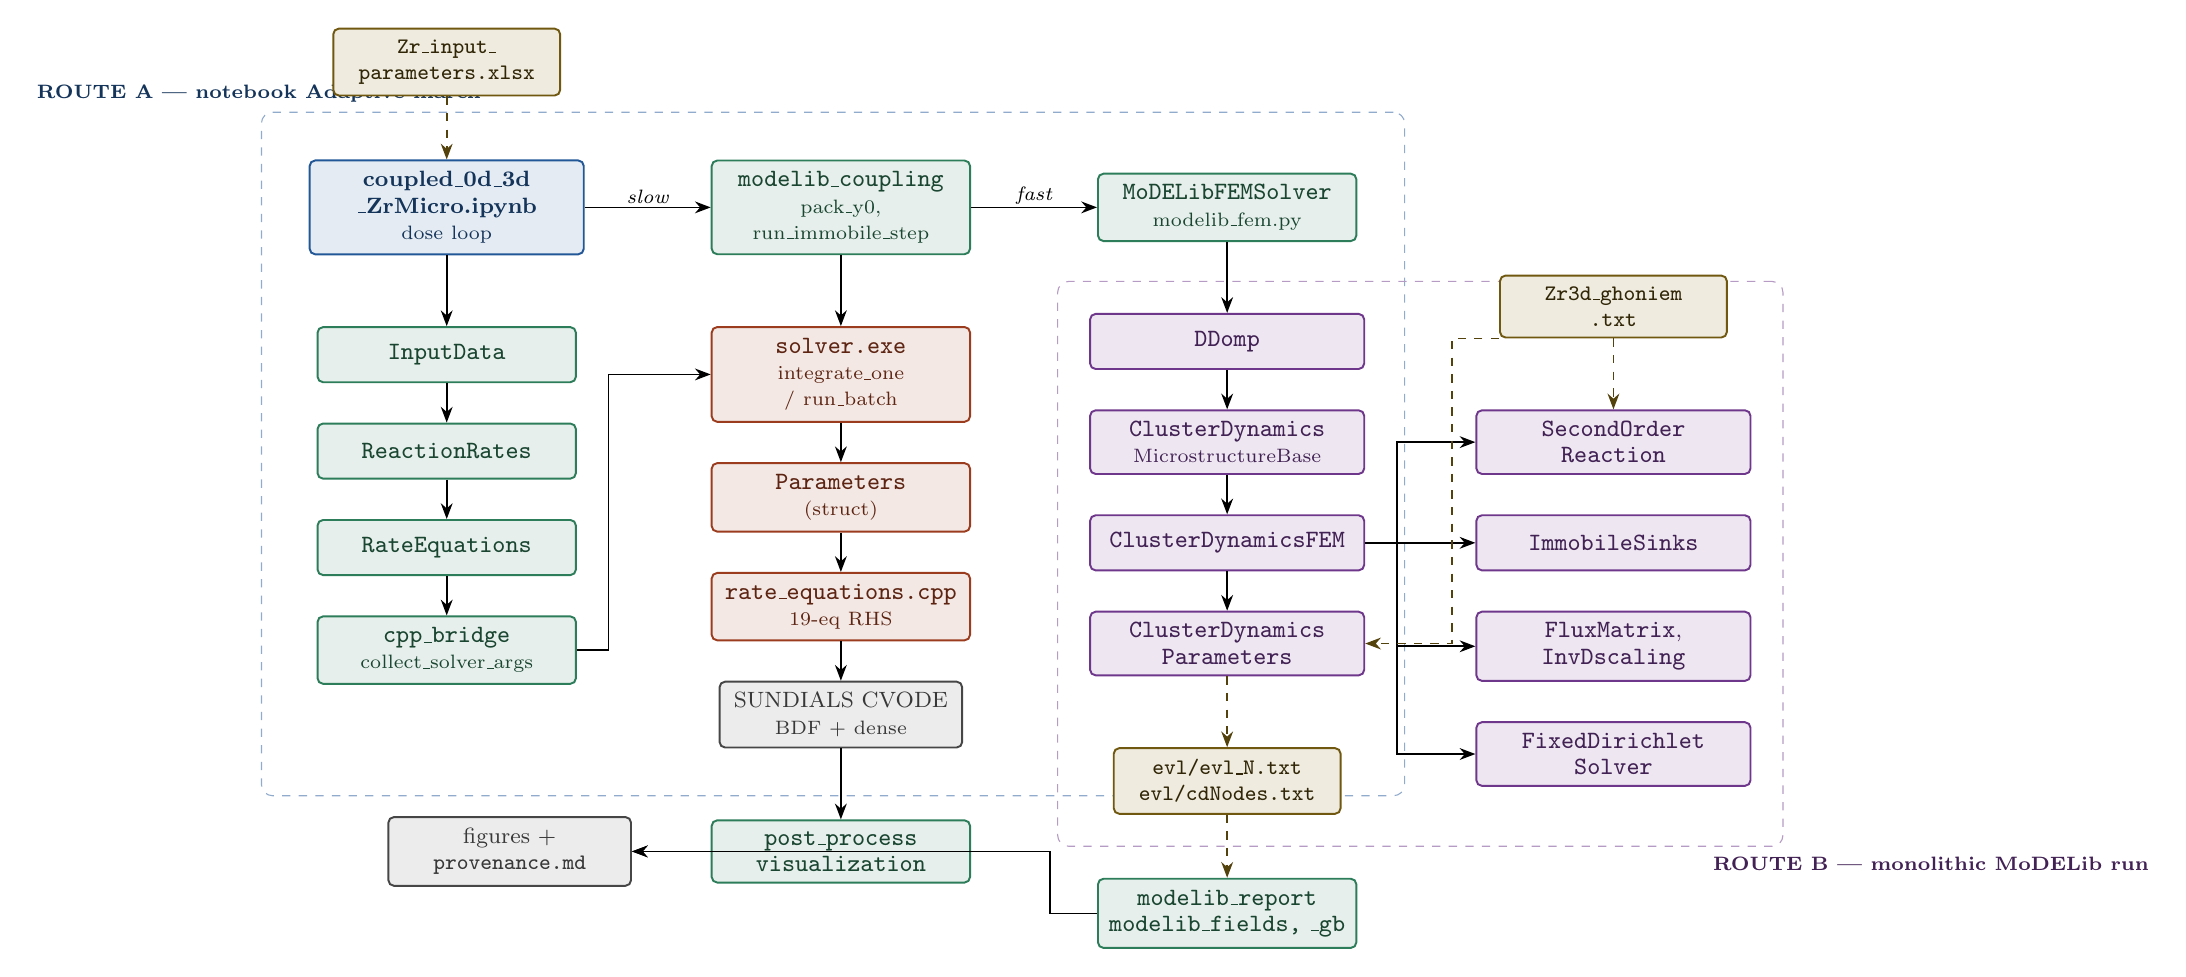
\begin{tikzpicture}[
  font=\footnotesize,
  node distance=5mm and 6mm,
  box/.style={draw, rounded corners=2pt, align=center, inner sep=4pt,
              minimum height=7mm, text width=#1, line width=0.7pt},
  nb/.style={box=32mm, fill=cNotebook!12, draw=cNotebook, text=cNotebook!60!black},
  py/.style={box=30mm, fill=cPy!12, draw=cPy, text=cPy!55!black},
  cpp/.style={box=30mm, fill=cCpp!12, draw=cCpp, text=cCpp!60!black},
  mod/.style={box=32mm, fill=cMod!12, draw=cMod, text=cMod!60!black},
  dat/.style={box=26mm, fill=cData!14, draw=cData!80!black, text=cData!35!black},
  prod/.style={box=28mm, fill=cOut!10, draw=cOut, text=cOut!80!black},
  call/.style={-{Stealth[length=2mm]}, line width=0.6pt},
  io/.style={-{Stealth[length=2mm]}, line width=0.6pt, dashed, draw=cData!60!black},
  lbl/.style={font=\scriptsize\itshape, inner sep=1pt}
]

% ---------------- column 1 : orchestration --------------------------------
\node[nb] (ipynb) {\textbf{coupled\_0d\_3d}\\\textbf{\_ZrMicro.ipynb}\\\scriptsize dose loop};
\node[dat, above=8mm of ipynb] (xlsx) {\file{Zr\_input\_}\\\file{parameters.xlsx}};
\node[py, below=9mm of ipynb] (idata) {\code{InputData}};
\node[py, below=of idata] (rrates) {\code{ReactionRates}};
\node[py, below=of rrates] (reqs) {\code{RateEquations}};
\node[py, below=of reqs] (bridge) {\code{cpp\_bridge}\\\scriptsize collect\_solver\_args};

% ---------------- column 2 : ZrMicro C++ ----------------------------------
\node[py, right=16mm of ipynb] (coup) {\code{modelib\_coupling}\\\scriptsize pack\_y0, run\_immobile\_step};
\node[cpp, below=9mm of coup] (solver) {\code{solver.exe}\\\scriptsize integrate\_one / run\_batch};
\node[cpp, below=of solver] (params) {\code{Parameters}\\\scriptsize (struct)};
\node[cpp, below=of params] (rhs) {\code{rate\_equations.cpp}\\\scriptsize 19-eq RHS};
\node[prod, below=of rhs] (cvode) {SUNDIALS CVODE\\\scriptsize BDF + dense};

% ---------------- column 3 : MoDELib --------------------------------------
\node[py, right=16mm of coup] (fem) {\code{MoDELibFEMSolver}\\\scriptsize modelib\_fem.py};
\node[mod, below=9mm of fem] (ddomp) {\code{DDomp}};
\node[mod, below=of ddomp] (cd) {\code{ClusterDynamics}\\\scriptsize MicrostructureBase};
\node[mod, below=of cd] (cdfem) {\code{ClusterDynamicsFEM}};
\node[mod, below=of cdfem] (cdp) {\code{ClusterDynamics}\\\code{Parameters}};

% ---------------- column 4 : MoDELib inner ---------------------------------
\node[mod, right=14mm of cdfem] (sinks) {\code{ImmobileSinks}};
\node[mod, above=of sinks] (r2) {\code{SecondOrder}\\\code{Reaction}};
\node[mod, below=of sinks] (flux) {\code{FluxMatrix},\\\code{InvDscaling}};
\node[mod, below=of flux] (fds) {\code{FixedDirichlet}\\\code{Solver}};
\node[dat, above=9mm of r2] (mat) {\file{Zr3d\_ghoniem}\\\file{.txt}};

% ---------------- outputs --------------------------------------------------
\node[dat, below=9mm of cdp] (evl) {\file{evl/evl\_N.txt}\\\file{evl/cdNodes.txt}};
\node[py, below=9mm of cvode] (post) {\code{post\_process}\\\code{visualization}};
\node[prod, left=10mm of post] (figs) {figures +\\\file{provenance.md}};
\node[py, below=8mm of evl] (mfld) {\code{modelib\_report}\\\code{modelib\_fields, \_gb}};

% ---------------- edges: orchestration -------------------------------------
\draw[io]   (xlsx)  -- (ipynb);
\draw[call] (ipynb) -- (idata);
\draw[call] (idata) -- (rrates);
\draw[call] (rrates)-- (reqs);
\draw[call] (reqs)  -- (bridge);
\draw[call] (ipynb) -- node[lbl,above]{slow} (coup);
\draw[call] (coup)  -- node[lbl,above]{fast} (fem);

% ---------------- edges: ZrMicro C++ ---------------------------------------
\draw[call] (coup)   -- (solver);
\draw[call] (bridge.east) -- ++(4mm,0) |- (solver.west);
\draw[call] (solver) -- (params);
\draw[call] (params) -- (rhs);
\draw[call] (rhs)    -- (cvode);

% ---------------- edges: MoDELib -------------------------------------------
\draw[call] (fem)   -- (ddomp);
\draw[call] (ddomp) -- (cd);
\draw[call] (cd)    -- (cdfem);
\draw[call] (cdfem) -- (cdp);
\draw[call] (cdfem) -- (sinks);
\draw[call] (cdfem.east) -- ++(4mm,0) |- (r2.west);
\draw[call] (cdfem.east) -- ++(4mm,0) |- (flux.west);
\draw[call] (cdfem.east) -- ++(4mm,0) |- (fds.west);
\draw[io]   (mat) -- (r2);
\draw[io]   (mat.south west) -- ++(-6mm,0) |- (cdp.east);

% ---------------- edges: products ------------------------------------------
\draw[io]   (cdp)  -- (evl);
\draw[io]   (evl)  -- (mfld);
\draw[call] (cvode) -- (post);
\draw[call] (post) -- (figs);
\draw[call] (mfld.west) -- ++(-6mm,0) |- (figs.east);

% ---------------- route annotations ----------------------------------------
\begin{scope}[on background layer]
\node[draw=cNotebook!50, dashed, rounded corners, fit=(ipynb)(coup)(fem)(bridge)(cvode),
      inner sep=6mm, label={[cNotebook!60!black,font=\scriptsize\bfseries]above left:ROUTE A
      --- notebook Adaptive march}] {};
\node[draw=cMod!50, dashed, rounded corners, fit=(ddomp)(cdp)(fds)(evl),
      inner sep=4mm, label={[cMod!60!black,font=\scriptsize\bfseries]below right:ROUTE B
      --- monolithic MoDELib run}] {};
\end{scope}

\end{tikzpicture}}
\caption{Component call graph. Solid arrows are calls, dashed arrows are
file input/output. Blue: orchestrating notebook; green: \ZrM{} Python; red:
\ZrM{} C++; purple: \MoD{} C++; ochre: files on disk; gray: products. Route
A drives the fast mobile solve through \MoD{} and the slow immobile march
through the \ZrM{} integrator; Route B runs both inside \MoD{}. The two
routes share the material definitions and the post-processing layer.}
\label{fig:flow}
\end{figure}

\subsection{Anisotropic diffusion and the discrete handoff}
\label{sec:aniso-handoff}

Two capabilities were added on 16 August 2026 and both change how a case is
set up, so they belong in the architecture rather than only in the change log.

\paragraph{One anisotropy factor, two representations.}
The diffusional anisotropy difference appears in the material file twice: as
\code{mobileSpeciesEnergyMigration\_eV}, the tensor the fast solve diffuses
with, and as \code{dadAnisotropy}, the $p_m$ that Woo's closed-form capture
efficiencies use. These used to be set independently, so the code could
simultaneously believe that diffusion was isotropic and that the sinks were
biased by its anisotropy. \file{staging/anisotropy.py} now generates both from
one $p_m$ per species, splitting the migration energy at fixed
$D_{\text{eff}}=(D_a^2 D_c)^{1/3}$ so that changing $p_m$ changes the
\emph{directionality} of diffusion and not its overall rate --- which is what
leaves the existing calibration intact:
\begin{equation}
E_m^{\langle 11,22\rangle}=E_m^{\text{eff}}+2k_BT\ln p_m,
\qquad
E_m^{\langle 33\rangle}=E_m^{\text{eff}}-4k_BT\ln p_m .
\end{equation}
Note the temperature dependence this introduces: because the anisotropy is
stored as energies, $p_m(T)=\exp(-\Delta E_m/6k_BT)$, so a pair fixed to give
0.7 at 573\,K gives 0.649 at 473\,K. That is physically right --- anisotropy
weakens as temperature rises --- and it repairs a fit previously frozen at one
temperature.

\paragraph{Which anisotropy to use.} Both loop-growth conditions reduce to
bounds on a single number, the arrival ratio
$A/B=\bar D_v c_v / \sum_m \bar D_m c_m |m|$, and the window between those
bounds is non-empty if and only if $p_I<p_v$. The measured co-growth set is
\begin{equation}
p_m=(p_v,p_i,p_{2i},p_{3i}) = (1.000000,\;0.913720,\;0.913720,\;0.913720),
\end{equation}
vacancies isotropic and the interstitials at the value \code{dadAnisotropy}
already carried, with tolerance $p_v\in[0.94,1.07]$. Two limits must be quoted
with any use of this: the criterion governs the \emph{absorption flux} only ---
the content update also carries cascade nucleation, which no anisotropy
affects --- and an isotropic march is not a zero of the criterion but simply
another parameter point, so a ratio taken against one cannot test a statement
about signs.

\paragraph{The handoff.} \file{post/coarsening.py} decides \emph{when} the
continuum description of a loop family stops being adequate, reporting
$d_{\text{coarsen}}$ where the Avrami overlap fraction crosses $\varphi^\ast$.
\file{coupling/transition.py} performs the switch at the next fast-solve
boundary, where a \code{DDomp} call happens anyway and the two sides are
already synchronized. It is armed by \code{COUPLING['discrete\_transition']}
and is \textbf{off by default}. Three invariants are audited across every
transfer: loop number, stored defects (exact to $10^{-16}$), and sink
strength --- the last of which \emph{jumps}, by design, and is reported rather
than asserted on.

Two practical constraints govern whether a transfer is possible at all.
\code{microstructureGenerator} silently refuses loops whose nodes leave the
grain, so \code{fits\_in\_crystal} predicts that decision and keeps the refused
share in the continuum; and the domain must be large enough to contain the
loops, which is not automatic. On the 500\,nm case the kept fraction is 0.997
at 0.1\,dpa and 0.55 from 1\,dpa onward, the latter a purely geometric plateau;
on the 200\,nm case it is exactly zero, because the basal radii reach 65\,nm
against a 173\,nm extent. \textbf{Check the kept fraction before trusting a
transfer on any new geometry.}

\subsection{Known non-correspondences between the 0-D and 3-D models}
\label{sec:noncorr}

These are physics, not bugs --- do not ``fix'' them silently:

\begin{enumerate}
\item \textbf{DAD bias.} The 0-D uses phenomenological anisotropy parameters
$\delta_i, \delta_v$ with $Z_a + Z_c = 2$; the 3-D generates the bias from
the diffusion tensors via $p_m$. They are reconciled by a closed-form fit of
$(Z^0_m, p_m)$ in \file{Zr3d\_ghoniem.txt}, valid only at the fitted
temperature. \file{Zr4.txt} is the standalone 3-D calibration and carries no
\code{dad*} keys --- do not check against it.
\item \textbf{Bi-pyramid vacancy family} --- exists only in the 3-D model.
\item \textbf{Size-dependent vacancy-loop thermal emission} --- 3-D only;
the 0-D uses a constant surrogate.
\end{enumerate}

%==============================================================================
\section{Changes relative to upstream MoDELib}
\label{app:changes}

\paragraph{Which upstream.} \textbf{The baseline is \file{mlm335/MoDELib2-NNL}},
at the point the immobile population equations were written into it. That code
solves the mobile steady-state PDE of Eq.~\eqref{eq:mobile} and nothing else:
its immobile species count is zero, \code{solveImmobileClusters()} is an empty
function body, and there is a literal \code{// Missing immobile sinks}
placeholder where the loop term would go. The loop populations were
\emph{absent}, not present in a simplified form, and the list below is stated
against that.

\file{mlm335/MoDELib-fullCD} is a \emph{separate} cluster-dynamics branch:
\code{iSize} is 8, it has its own immobile integrator
(\file{ImmobileSinkRate.h}, \file{SpatialODESolver.h}), the loop sink on the
mobile species (\file{FirstOrderReaction.h}), and a continuum-to-discrete loop
conversion that \MoD{} does not have. It is a sibling, not the ancestor.

\paragraph{A correction.} An earlier revision of this manual declared fullCD the
correct baseline and \MoD{}'s immobile solver a \emph{re-discretization} of its
scheme, on the evidence that 31 cluster-dynamics parameter keys are shared
verbatim and most of the rest are systematic renames. \textbf{That inference
does not follow.} Shared naming across two branches of one code, developed in
one group from one formulation, is evidence of \emph{convergence} and says
nothing about which came first. The immobile equations here were written to
reproduce ZrMicro, not to re-express fullCD. A full numbered history is given in
the companion note \file{DisloCluster Code History}.

The two schemes remain worth comparing as siblings, and differ in the
discretization: fullCD projects its rate through the consistent mass matrix and
takes one explicit-Euler step of \code{dtMax} followed by sequential implicit
loss factors, where \MoD{} evaluates the rate at nodes and takes 20 sub-steps of
a single fused semi-implicit update.

Relative to \file{MoDELib2-NNL} the entire immobile half of the model is new.
The following are the pieces of it, with the sibling comparison noted where one
exists:

\begin{itemize}
\item the loop density and content evolution equations
(\code{solveImmobileClusters()}), re-discretized as above;
\item homogeneous SIA-clustering nucleation, read off the reaction network
the mobile solve already uses (\code{getLoopNucChannels()});
\item the loop absorption sink on the mobile species
(\file{ImmobileSinks.h}), deliberately excluding the grain boundary, which
the spatially resolved model captures through the Dirichlet condition and
would otherwise be counted twice;
\item DAD capture efficiencies from $(p_m, Z^0_m)$ (\code{loopDADbias()});
\item absorption fluxes with cluster weighting, the minimum-stable-size
gate, vacancy-loop dissolution, size-dependent thermal vacancy emission, and
two-channel Avrami coalescence;
\item a screened cutoff on the Galerkin climb pair assembly, through the
optional material key \code{climbNeighborCutoff\_b}. The assembly runs over
every ordered pair of segments and is 100\% of the climb-solve cost --- the
live path is lumped, so its ``solve'' is one scalar division per node.
Truncation is legitimate because the kernel is not bare $1/r$ but screened as
$e^{-kr}/r$ by the same $k^2$ \file{ImmobileSinks.h} already assembles, and
because the continuum field already carries the mean-field response of the
whole population, so the discrete sum must supply only the near-field
correction. Zero or absent means no cutoff, so every material file written
before the key existed is unaffected; an enormous cutoff reproduces the uncut
assembly bit-for-bit. The measured truncation error on the basal
plastic-distortion rate is 19.3\%, 9.6\%, 3.9\% and 0.25\% at
$R_c/L_s$ of 1, 2, 3 and 4 respectively, so the default is \textbf{4}.
\end{itemize}

Four defects were also corrected in pre-existing upstream code: a
member-initialization-order bug that silently dropped the Boltzmann factor
from the cluster dissociation rates; a spurious scaling of the diffusion
operator relative to the reaction terms after the cluster-dynamics atomic
volume became independently settable; a unit error that left the
minimum-stable-radius gate permanently open; and the use of the two-atom
hexagonal lattice \emph{cell} volume where the atomic volume was intended
(now settable explicitly via the optional \code{atomicVolume\_SI} material
key).

On the input side, Po's standalone calibration \file{Zr4.txt} is left
untouched; the coupled, reconciled definition is the separate file
\file{Zr3d\_ghoniem.txt}, which resets the mobile block (cascade fractions,
migration energies, diffusivities, reaction prefactors, network sink) to
correspond with the 0-D model and adds the entire immobile block ($\sim$20
new keys). The full before-and-after, key by key, is in
\file{MoDELib3/ZR3D\_GHONIEM\_CHANGES.md} and in the companion architecture
document.

%==============================================================================
\section{Quick reference}
\label{app:quickref}

The complete sequence from a fresh Windows machine to figures, assuming the
prerequisites of Section~\ref{sec:install} (Git, Python 3.14, VS Build
Tools, CMake, WSL + Ubuntu, SUNDIALS in \file{Libraries/}) are in place. All
commands from the repository root.

\begin{lstlisting}[style=ps]
# 1. clone
PS> git clone https://github.com/Ghoniem/DisloCluster.git ; cd DisloCluster

# 2. python environment + kernel
PS> C:\Python314\python.exe -m venv .DisloClusterVenv
PS> .DisloClusterVenv\Scripts\python.exe -m pip install -r requirements.txt
PS> .DisloClusterVenv\Scripts\python.exe -m ipykernel install --user `
      --name dislocluster --display-name "Python 3.14 (DisloCluster)"

# 3. verify path resolution (repeat after each build)
PS> .DisloClusterVenv\Scripts\python.exe dislocluster_code\paths.py

# 4. build the 0-D solver (native Windows)
PS> cmake -S ZrMicro\cpp_utils -B ZrMicro\build `
      -DCMAKE_BUILD_TYPE=Release
PS> cmake --build ZrMicro\build --config Release

# 5. build the 3-D code (inside WSL; note the explicit MoDELib3 argument)
PS> wsl -u root -e bash Docs/Formulation/build_modelib.sh MoDELib3

# 6. first test: figures from the shipped 3-D results (minutes)
PS> .DisloClusterVenv\Scripts\python.exe `
      dislocluster_code\studies\run_zr3d_singlecrystal.py `
      --doses 1 5 10 30 --max-nm 150

# 7. the full 3-D solve (hours) -- then rerun step 6
PS> wsl -e bash MoDELib3/tutorials/zrmicro_coupled/clean_run.sh

# 8. the 0-D model (minutes)
PS> .DisloClusterVenv\Scripts\python.exe -m nbconvert --to notebook --execute `
      --ExecutePreprocessor.kernel_name=dislocluster `
      --output-dir Simulations\output `
      ZrMicro\code\ZrMicro.ipynb

# 9. the coupled 0-D <-> 3-D march (open interactively, or:)
PS> .DisloClusterVenv\Scripts\python.exe -m nbconvert --to notebook --execute `
      --ExecutePreprocessor.kernel_name=dislocluster `
      --output-dir Simulations\output `
      ZrMicro\code\coupled_0d_3d_ZrMicro.ipynb
\end{lstlisting}

\noindent Key locations:

\begin{table}[htbp]
\centering
\begin{tabular}{@{}ll@{}}
\toprule
what & where \\
\midrule
path resolution (run it!) & \file{dislocluster\_code/paths.py} \\
0-D inputs & \file{Simulations/input/Zr\_input\_parameters.xlsx} \\
3-D material file & \file{MoDELib3/Library/Materials/Zr3d\_ghoniem.txt} \\
3-D case inputs & \file{MoDELib3/tutorials/zrmicro\_coupled/inputFiles/} \\
all outputs & \file{Simulations/output/} \\
env overrides & \code{DISLOCLUSTER\_ROOT}, \code{MODELIB\_ROOT}, \code{MODELIB\_BUILD} \\
\bottomrule
\end{tabular}
\end{table}

\end{document}
